% user-input-script.tex
\newpage
\section{Input Script Overview}
Currently, \texttt{e3prep.py}\index{e3prep.py} is implemented as 
a Python program that has a library of classes specialized for constructing
geometric regions and specifying flow conditions.
Because your specification script, \texttt{{\em job}.py}, 
becomes a part of that program when it runs,
it is worth the effort to learn just enough Python to be dangerous.
The web site \url{http://www.python.org} is a good starting point for
learning about the Python programming language, however, Appendix\,\ref{python-notes-sec}
may have enough information to get you started.

\medskip
After doing some initialization, \texttt{e3prep.py} executes your
script file and assembles the geometry and flow specification data
into a form that can be given to the main simulation code
\texttt{e3shared.exe}\index{e3shared.exe}\footnote{The ``shared'' tag indicated that we are
  using the shared-memory version of the code.  
  There is also a distributed-memory version, \texttt{e3mpi.exe}\index{e3mpi.exe},
  based on message passing (MPI) that can be used for running the main simulation.
}.
The advantage of this approach is that you have the full capability of 
the Python interpreter available to you from within your script.
You can perform calculations so that you can parameterize your geometry, 
for example, or you can use Python control structures
to make repetitive definitions much more concise.
Additionally, you may use Python comments and print statements
to add documentation to the script file. 
An input script usually does the following:
\begin{enumerate}
  \item selects gas model
  \item optionally, creates geometric elements to assist in defining the boundary representation of the gas domain
  \item creates blocks within the gas domain and specifies their discretization and, optionally, 
        specifies boundary conditions along some block surfaces (in 3D) or edges (in 2D)
  \item specifies remaining boundary conditions, if any
  \item sets some simulation control parameters
\end{enumerate}
Most examples in this manual do just these things, however, it is possible to do much more.
The example that computes the heat transfer to a sphere (Section\,\ref{sphere-heat-transfer-sec}) uses a top-level Python
script to coordinate a number of simulations with increasingly-refined grids as a crude multigrid simulation.

\clearpage

\medskip
To aid with debugging, it is easy to process part of your input script and
then temporarily put the interpreter into an interactive mode where 
you may type python commands and expressions at the prompt (\texttt{>>>}).
To do so, add the following lines at the appropriate point in your input
script.\\
%
\topbar\\
\texttt{from code import interact}\index{e3prep.py!interactive mode}\\
\texttt{interact('Start interactive mode (Ctrl-D to return)', local=locals())}\\
\bottombar\\
%
Now you can interact with the Python environment and the objects that your
input script has defined so far.
For example, to find out a bit about defining \texttt{Block3D} objects, type:\\
%
\topbar\\
\texttt{>>> help(Block3D)}\\
\bottombar\\
%
To get out of the interactive mode and continue processing the input script,
type \texttt{Control-D} at the prompt.


%------------------------------------------------------------------
\section{Thermochemical model and flow conditions}
\label{thermo-flow-sec}\index{thermochemical models}\index{module!libgas}
%
The thermochemical models are provided by the \texttt{libgas} module.
This is primarily a C++ module but it has a SWIG-generated Python interface so
that its objects and methods can be accessed from the user's input script.

\subsection{10 second version: just tell me how to select perfect air}
Place the following text (which is a function call) in your script \emph{before}
specifying any \texttt{FlowCondition} objects:\\
%
\topbar\\
\texttt{select\_gas\_model(model='ideal gas', species=['air'])}\\ \index{select\_gas\_model}
\bottombar\\
%
If this is the only gas model that interests you for the present, then
proceed to page~\pageref{sec:flow_condition} which discusses the specification
of a \texttt{FlowCondition}.

\subsection{2 minute version: tell me about other simple models}

To select a gas model, the user calls the function
\texttt{select\_gas\_model}.
This function accepts three keyword arguments: \texttt{model},
\texttt{species}, and \texttt{fname}.
In the vast majority of cases, only the first
two keyword arguments will be used.
This function must be called \emph{before} specifying any \texttt{FlowCondition} objects
so that the complete thermodynamic state can be computed.

\medskip
A second example: to select an ideal mixture of nitrogen and oxygen
call:\\
%
\topbar\\
\texttt{select\_gas\_model(model='ideal gas', species=['N2', 'O2'])}\\
\bottombar\\
%
Note that the only difference between selecting a mixture and a single
component gas is the addition of extra species in the species list and the extra computation that
the main simulation program needs to do.

\medskip
In general, the \texttt{model} keyword accepts a string describing
the gas model behaviour.
The available gas models are:
\begin{itemize}
 \item \texttt{'ideal gas'}: a gas with ideal behaviour: modelled as having perfectly elastic collisions
                             and constant specific heats\index{gas model!ideal}
 \item \texttt{'thermally perfect gas'}: a gas with thermally perfect behaviour: modelled as having perfectly
                             elastic collisions but with specific heats that are functions of temperature
                             \index{gas model!thermally perfect}
% \item \texttt{'one temperature gas'}: similar to the 'thermally perfect gas' except that the thermodynamic 
%                             properties are calculated from statistical mechanics rather than the CEA curve 
%                             fits\footnote{Due to the assumption of decoupled thermal modes, the thermodynamic
%                             properties for the 'one temperature gas' model are not as accurate as the CEA curve
%                             fits.  The purpose of the this gas model is to provide a single temperature 
%                             equivalent of the multiple temperature gas models.  For general thermal equilibrium
%                             calculations, users are advised to use the 'thermally perfect gas' model.}, and
%                             transport properties are calculated via collision-integrals.
 \item \texttt{'two temperature gas'}: a thermally perfect gas\footnote{The two temperature gas model is thermally
                             perfect in the sense that the thermodynamic properties are functions
                             of temperature only, however multiple temperatures are defined.} with two independent
                             thermal modes: one temperature $T_\text{tr}$ governs the heavy-particle translation 
                             and rotation modes, and another temperature $T_\text{ve}$ governs the vibration, 
                             electronic and free-electron translation modes.
                             \index{gas model!two temperature}
% \item \texttt{'three temperature gas'}: a thermally perfect gas with three independent thermal modes: the 
%                             temperature $T_\text{tr}$ governs the heavy-particle translation and rotation modes,
%                             $T_\text{v}$ governs the vibration modes and $T_\text{e}$ governs the
%                             electronic and free-electron translation modes.
%                             \index{gas model!three temperature}
% \item \texttt{'four temperature gas'}: a thermally perfect gas with four independent thermal modes: the 
%                             temperature $T_\text{t}$ governs the heavy-particle translation modes, $T_{\text{r}}$
%                             governs the rotation modes, $T_\text{v}$ governs the vibration modes and $T_\text{e}$ 
%                             governs the electronic and free-electron translation modes.
%                             \index{gas model!four temperature}
 \item \texttt{'real gas Bender'}: a gas with real behaviour, such as accurate thermodynamic property evaluation
                            at high density and pressure near the saturation boundary and in the critical region.
                            This model is based on the Bender \textit{p-v-T} relationship.
                             \index{gas model!real gas!Bender}
 \item \texttt{'real gas MBWR'}: a gas with real behaviour, such as accurate thermodynamic property evaluation
                            at high density and pressure near the saturation boundary and in the critical region.
                            This model is based on the MBWR \textit{p-v-T} relationship, which is more accurate
                            than the Bender \textit{p-v-T} relationship.
                             \index{gas model!real gas!MBWR}
 \item \texttt{'real gas REFPROP'}: a gas with real behaviour, such as accurate thermodynamic property evaluation
                            in all single and two phase regions.
                            This model makes use of the REFPROP thermodynamic database and is more accurate than
                            the MBWR gas model.
                             \index{gas model!real gas!REFPROP}
\end{itemize}

The \texttt{species} keyword accepts a list of strings; each string denotes
a species in the mixture.  The order of this list is important: the order of
species in this list corresponds to the order in which the species mass fractions
are specified in other parts of the input.
To get a list of available species, look at the selection of species which are placed
in the \texttt{\$HOME/e3bin/species}\index{species!list of available} area during the install, 
that is, at a command prompt type:

\noindent
\topbar\\
\texttt{> ls \$HOME/e3bin/species}\\
\bottombar\\
%
The names of these files (excluding the \texttt{.lua} extension) correspond to the
names of available species.  The \texttt{defaults.lua} file is not a species name.
Rather, this file provides a set of default values when no other data is available.

\subsection{Specifying the gas model with \texttt{gasmodel.py}}
Since the gas model module gets all its information about the gas from an external
file (typically called \texttt{gas-model.lua}), it is reasonable to prepare the gas
model specification external to your input script.
To assist with this process, the program \texttt{gasmodel.py} is available.
Running this program without specifying any options provided the following usage message:

\noindent
{\footnotesize
\begin{verbatim}
$ gasmodel.py 

Use this program to construct a simple or composite gas model for use with
the simulation codes Eilmer3 of L1d3.

Usage: 
  gasmodel.py [--help] [--model=<modelName>] [--species=<speciesList|none>] \
              [--lut-file=<LUTFileName>] \
              [--output=<luaFile|gas-model.lua>]

Input parameters:
  model   : name of the gas model, may have embedded spaces.
  species : list of species names (space delimited) in a single string.
  output  : name of the gas-model file to be written.
  lut-file: name of the preexisting LUT-gas model file, if relevant.

Examples:
  $ gasmodel.py --model='thermally perfect gas' --species='N2 N' \
                --output='nitrogen.lua'

  $ gasmodel.py --model='ideal gas' --species='Ar He' \
                --lut-file='cea-lut-custom.lua.gz' \
                --output='LUT-plus-Ar-He.lua'

Notes:
  If you want a LUT-plus-composite gas model, set up the LUT table
  externally. Invoke this program, specifying the rest of the species
  for the composite gas model.  The LUT gas species is prepended to 
  the composite gas species list.  You will need both gas model files
  in place to use the resulting LUT-plus-composite gas model.
\end{verbatim}
} % end footnotesize

\noindent
Once you have your gas-model file generated, just give its file name to 
the \texttt{select\_gas\_model} function call in your input script.

\subsection{10 minute version: the detail of gas model configuration}
In the earlier examples, the \texttt{select\_gas\_model} function was called using
the two keyword arguments \texttt{model} and \texttt{species}.
Behind the scenes, this function calls an auxiliary set of tools to build
a stand-alone text file which is a configuration file for the gas model.
This configuration file is a Lua-style file: it is read directly by the
C++ code (with embedded Lua interpreter) in order to configure the gas model.
By default, the created configuration file is called \texttt{gas-model.lua}.
This file will sit in your working directory after a successful call to
\texttt{select\_gas\_model} using only the \texttt{model} and \texttt{species} keyword
arguments.
The configuration file contains all the necessary details to completely
specify the gas.
Thus, this file serves as a record of the gas model input parameters used in
your simulation.

\medskip
You are encouraged to open the file \texttt{gas-model.lua} and take a look.
It contains not only the input parameters for the gas model but also references for the
data where possible.
Some amount of effort has been made to design a configuration file that
properly documents the input data.
The use of Lua as the configuration language has aided this effort.

\medskip
Alternatively, the \texttt{select\_gas\_model} function may also be called
with \texttt{fname} as a keyword argument.
This argument, \texttt{fname}, accepts a string which names a Lua-style configuration
file for the gas model.
Thus, if you have a gas model configuration file from a previous simulation, you could
set the gas model with the call:\\
%
\topbar\\
\texttt{select\_gas\_model(fname='gas-model.lua')}\\
\bottombar\\
%
This assumes your configuration file is called \texttt{gas-model.lua} and resides
in the same directory as your main simulation script.\index{gas model!gas-model.lua file}

\medskip
Finally, for certain advanced gas models (such as a gas with multiple vibrational temperatures),
the only means to configure these models is via the preparation of a Lua-style configuration
file by hand.
After building a file by hand (that is, in a text editor), one would use the \texttt{fname} keyword
argument in the call to \texttt{select\_gas\_model} to set the gas model.
The list of gas models which are set by directly creating a configuration file includes:
\begin{itemize}
 \item user-defined gas (by specification of callable Lua functions)\index{gas model!user-defined}
 \item an equilibrium gas, based on a look-up table\index{gas model!look-up table}
 % DFP: this model is specified via 'thermally perfect gas'
 % \item a reacting mixture of thermally perfect gases\index{gas model!reacting}
\end{itemize}
Further discussion of gas models which are set by direct creation
and manipulation of a configuration file is given in Appendix~\ref{app:gas-models}.

\subsection{Selecting a simple model and adjusting it}
The simple ideal gas model of air as discussed above has $\gamma = 1.4$.
You can get an air model with $\gamma = 1.3$ by selecting the species
as \texttt{'air13'} or you can adjust the value of $\gamma$ directly
for the ideal gas model.
This can be done from within the Python input script by calling the function 
\texttt{change\_ideal\_gas\_attribute()},\index{gas model!change\_ideal\_gas\_attribute}
and telling it which species, which attribute and what new value to use.
The function actually does a string substitution within the \texttt{gas-model.lua} file
that was generated behind the scenes when the \texttt{select\_gas\_model()} function was called.

\medskip
For an example of use, see the MNM Implosion problem in Section\,\ref{mnm-implosion-sec}.
There, the value of ratio of specific heats is changed with the lines\\
%
\topbar\\
\texttt{gas\_gamma = 5.0/3.0}\\
\texttt{select\_gas\_model(model='ideal gas', species=['air'])}\\
\texttt{change\_ideal\_gas\_attribute('air', 'gamma', gas\_gamma)\\}
\bottombar\\
You might also like to change the gas constant but, since that is not an actual parameter in the 
\texttt{gas-model.lua} file, it needs to be set indirectly, via the molecular mass (in units of kg/mol).\\
\topbar\\
\texttt{Rgas = 300.0}\\
\texttt{MM = R\_u / Rgas}\\
\texttt{change\_ideal\_gas\_attribute('air', 'M', MM)\\}
\bottombar\\
Note that \texttt{'M'} is the label for molecular mass in the \texttt{gas-model.lua} file
and \texttt{R\_u} is the universal gas constant made available by the thermochemistry module
to the Python input script.


\subsection{Specifying chemically reacting flow}
\index{chemical reaction!reaction scheme file}
For chemically reacting flow simulations, the following function call is
required:\\
%
\topbar\\
\texttt{set\_reaction\_scheme(config\_file, reacting\_flag=1, T\_frozen=300.0)}\\
\bottombar\\
where \texttt{config\_file} is a string naming the configuration file for the
chemical reaction scheme.  This configuration file specifies all of the chemical
reactions between the various species and is built by hand by the user.\index{chemical reaction}
By default, the reactions are turned on, however, the user may elect to turn off
chemical reaction updates by setting \texttt{reacting\_flag=0}.
At low temperatures, it is unlikely that the reactions will proceed in any significant way
so you may set value of temperature, \verb!T_frozen!, below which the reaction updates will
be skipped.
This is checked on a cell-by-cell basis.

\medskip
Generally, you should use the \verb!'thermally perfect gas'! mix for all reacting flow simulations.
The enthalpies of formation are implicit in the enthalpy evaluation provided by the NASA Glen curves,
thus providing the proper effect of heat release due to rearrangement of chemical bonds.
Note that, at low temperatures, the ideal gas behaviour should be recovered so you shouldn't need 
to resort to using the \verb!'ideal gas'! model.

\medskip
An example of a reacting flow simulation is given in Section~\ref{sec:n90}.
The details of building a chemistry input file are provided in Appendix~\ref{app:chem}.

\subsection{Specifying thermal energy exchange mechanisms}
\index{thermal nonequilibrium!energy exchange scheme file}
For flow simulations where the number of thermal modes is greater than one (such as for the 
`two temperature gas' model previously
mentioned), energy exchange mechanisms can be defined that describe the exchange of thermal
energy between modes due to particle collisions.
If such energy exchange mechanisms wish to be modelled, the following function call is
required:\\
%
\topbar
\begin{verbatim}
set_energy_exchange_scheme(config_file, energy_exchange_flag=1, 
                           T_frozen_energy=300.0)\end{verbatim}
\bottombar\\
where \texttt{config\_file} is a string naming the Lua configuration file for the
energy exchange scheme.  This configuration file specifies all of the energy exchange 
mechanisms between the thermal modes due to thermal processes (i.e. particle collisions) 
and is built by hand by the user.\index{thermal energy exchange}
Thermal energy exchange is, by default, turned on when the
\texttt{set\_energy\_exchange\_scheme(config\_file)} function call is made, however,
you may restrict the exchanges to the zones where chemical reactions are allowed and you
can also set the temperature below which the exchanges will be skipped on a per-cell, per-timestep basis.

\medskip
An example of a flow simulation with thermal energy exchange is given in
Section~\ref{sec:finite-cyl-sec}.
The details of building a thermal energy exchange input file are provided in 
Appendix~\ref{app:therm-exchange}.

\subsection{Defining flow conditions}
\label{sec:flow_condition}
Because \texttt{Eilmer3} is a flow \textit{simulation} code, initial gas flow conditions
need to be specified throughout the domain.
Also, depending on your model, free-stream inflow boundary conditions 
may need to be specified on appropriate boundary surfaces.
To define such a flow condition in your input script for one or both of these purposes, 
create a \texttt{FlowCondition} object\footnote{The \texttt{FlowCondition} class is
  defined in source file \texttt{e3\_flow.py}} as:
\texttt{
\begin{tabbing}
my\_flow = FlowCondition(\=p=1.0e5, u=0.0, v=0.0, w=0.0, \\
                         \>Bx=0.0, By=0.0, Bz=0.0, T=[300.0,], \\
                         \>massf=None, label="", tke=0.0, omega=1.0, \\
%                         \>sigma\_T=0.0, sigma\_c=0.0, 
                         \>S=0, add\_to\_list=1)
\end{tabbing}
}\index{FlowCondition}\index{FlowCondition!add\_to\_list parameter}

%
\begin{itemize}
  \item \texttt{p}: pressure in Pa, default value 100\,kPa.
  \item \texttt{u}: $x$-coordinate velocity in m/s, default value 0.0.
  \item \texttt{v}: $y$-coordinate velocity in m/s, default value 0.0.
  \item \texttt{w}: $z$-coordinate velocity in m/s, default value 0.0.
  \item \texttt{Bx}: $x$-coordinate magnetic field in Tesla, default value 0.0.
  \item \texttt{By}: $y$-coordinate magnetic field in Tesla, default value 0.0.
  \item \texttt{Bz}: $z$-coordinate magnetic field in Tesla, default value 0.0.
  \item \texttt{T}: list of temperatures in degrees K, default value [300.0,].
    For gas models with multimodal energies, these are the corresponding temperatures.
    For a gas model with only one internal energy mode, you may specify a scalar value
    for temperature.
  \item \texttt{massf}: mass fractions of the component species.
    These may be provided in a number of ways:
    \begin{itemize}
      \item[(a)] full list of floats. The length of the list of mass fractions 
         must match the number of species in the previously selected gas model.
      \item[(b)] single float or integer that gets used as the first element,
         the rest being set 0.0
      \item[(c)] dictionary of species names with mass fraction values,
         the remainder being set 0.0.  See the example in Section\,\ref{sec:MoleFractions}.
      \item[(d)] None provided, results in the first element being 1.0
         and the rest 0.0
    \end{itemize}
    Note that the mass fractions supplied must sum to 1.0 (within a tolerance of $1.0 \times 10^{-6}$.
  \item \texttt{label}: (optional) text label for the FlowCondition object.
  \item \texttt{tke}: turbulent kinetic energy per unit mass in m$^2$/s$^2$ or
    J/kg, default value 0.0.
  \item \texttt{omega}: turbulence vorticity in 1/s, default value 1.0.
  \item \texttt{mu\_t}: turbulence viscosity in Pa.s, default value 0.0.
  \item \texttt{k\_t}: turbulence thermal conductivity, default value 0.0.
     This might be conveniently computed as $C_p \mu_t / Pr_t$.
%  \item \texttt{sigma\_T}: variance of temperature variations, default value 0.0.
%  \item \texttt{sigma\_c}: variance of species concentrations, default value 0.0.
  \item \texttt{S}: integer shock indicator value, default value 0.
    A value of 1 indicates the presence of a shock through the cell.
  \item \texttt{add\_to\_list}: flag to indicate that this FlowCondition object 
    should be added to the flowList.  Sometimes we don't want
    to accumulate objects in this list, for example, when using
    many FlowCondition objects in a user-defined flow evaluation function.
    default value 1.
\end{itemize}

\medskip
Simulations involving nonequilibrium chemistry require and extra input file
describing the participating gas species and their reactions.
Preparation of this file is described in Appendix\,\ref{app:chem}.

\subsection{Using flow conditions from other simulations}
\label{sec:ExistingSolution}
%
There are occasions where you might like to use flow data from an old simulation
as initial conditions for some or all of your blocks in your new simulation.
A typical use case is to restart a simulation with a finer, or otherwise changed, mesh.
For this, you may pick up the old simulation data using:\\
\index{ExistingSolution}
\texttt{
\begin{tabbing}
old\_flow = ExistingSolution(\=rootName, solutionWorkDir, nblock, tindx, \\
                             \>dimensions=2, assume\_same\_grid=0, zipFiles=1, \\
                             \>add\_velocity=Vector(0.0,0.0,0.0))\\
\end{tabbing}
}\index{ExistingSolution}
where the arguments and their possible values are:
\begin{itemize}
  \item \texttt{rootName}: job name that will be used to build file names
  \item \texttt{solutionWorkDir}: the directory where we'll find our existing solution files.
  \item \texttt{nblock}: number of blocks in the existing solution data set
  \item \texttt{tindx}: the time index to select 0..9999.
            Do not specify with leading zeros because the Python interpreter
            will assume that you want to count the time index in octal.
  \item \texttt{dimensions}: number of spatial dimensions for the existing solution
  \item \texttt{assume\_same\_grid}: decide how to locate corresponding cells
     \begin{itemize}
        \item[\texttt{0}]: searches for corresponding cells. This steps through each cell and
		searches for closest corresponding cell centre in the old solution and inserts
		the flow data.
                As Rainer found, this can be agonisingly slow for large grids.\index{Kirchhartz}
        \item[\texttt{1}]: omits the search for the corresponding cell.
                Definitely the option for the impatient. This assumes the same grid for the old and
		new solution and inserts flow data based on the i and j cell references.
     \end{itemize}
   \item \texttt{zipFiles}: to use gzipped files (1), or not (0)
   \item \texttt{add\_velocity}: value to be added to each cell's velocity,
       for changing frame of reference.
\end{itemize}
The process of writing the data into each cell of the new grid uses a fairly naive search for the 
nearest cell in the existing solution.
Although it is robust, the search is extremely slow and the preparation of sew grids has been known
to take hours of CPU time.
If the new simulation is a continuation of the old simulation, it may be appropriate to set
\texttt{gdata.t0} to a nonzero value.  See Section\,\ref{sec:sim-control-parameters}.

\subsection{Using mole fractions and species dictionaries}
\label{sec:MoleFractions}
%
When simulating flows with mixes of gas species, it may be more convenient to specify the gas mix
via mole fractions rather than mass fractions and via a dictionary rather than a list.
With large numbers of species in the gas model, specification of the mix via dictionary is far easier to
read and check than when using a list of numerical values. 

\medskip
There are a number of functions attached to the \texttt{Gas\_model} object that make the
conversion to a list of mass fractions easy.
Here is an extract from Umar's standing-shock script showing the creation of a fairly complex gas mix
using a dictionary of mole fractions.

\medskip\noindent\topbar
{\small %\scriptsize
\begin{verbatim}
select_gas_model(model='thermally perfect gas', 
                 species=['O', 'N', 'N2', 'O2', 'NO', 'N_plus', 'O_plus', 'N2_plus',
                          'O2_plus', 'NO_plus', 'e_minus', 'Ar', 'Ar_plus'])
set_reaction_scheme("gupta_etal_air_reactions.lua", reacting_flag=1)
gmodel = get_gas_model_ptr()

# Pre-shock gas: mass fractions for an ideal air mixture.
mi = {'N2':0.769, 'O2':0.231}
# Post-shock: mole fractions from a CEA calculation.
X = {'O':1.6936e-1, 'N':5.9784e-1, 'N2':6.9757e-5, 'O2':4.7543e-8, 'NO':2.5654e-3, 
     'N_plus':9.6331e-2, 'O_plus':1.7562e-2, 'N2_plus':7.7688e-6, 'O2_plus':5.0837e-8, 
     'NO_plus':1.4459e-5, 'e_minus':1.1436e-1, 'Ar':4.0026e-3, 'Ar_plus':4.4835e-4}

initial = FlowCondition(p=2700.0, u=0.0, v=0.0, T=300.0, massf=mi)
inflow  = FlowCondition(p=4464.0, u=10284.0, v=0.0, T=10140.42,
                        massf=gmodel.to_massf(X))
\end{verbatim}
}
\noindent\bottombar

%------------------------------------------------------------------
\section{Radiation transport model}
\label{radiation-transport-sec}
\index{radiation transport model!definition in input script}
%
The selection of a radiation transport model and the definition of its parameters
is done in a Lua file.
The format for the Lua file describing the radiation transport model is give in Appendix~\ref{app:rt-models}.
A radiation model is brought into an Eilmer3 simulation via the \texttt{select\_radiation\_model} function:

\noindent\topbar\\
\texttt{select\_radiation\_model( input\_file=None, update\_frequency=1, scaling=True )} 
\index{select\_radiation\_model} \\
\bottombar\\

The input variables are:

\begin{description}
 \item[ \texttt{input\_file}] The name of the Lua file with the radiation transport and spectral model definitions (defaults to \texttt{None})
 \item[\texttt{update\_frequency}] Number of time steps between re-calculation of the radiation solution (defaults to \texttt{1})
  \item[\texttt{scaling}] Flag to request scaling of stored radiation solution based on density and temperature for time steps where the radiation solution is not re-calculated due to the update frequency being greater than 1 (defaults to \texttt{True})
\end{description}
 

For example, the following entry in the Eilmer input script requests the radiative source terms and heat fluxes
 to be recomputed every 100 time steps with scaling between recomputed solutions and directs \texttt{e3prep.py} to the file \texttt{rad-model.lua} 
 for the details of the desired radiation transport and spectral modelling:

\noindent\topbar\\
\texttt{select\_radiation\_model( input\_file="rad-model.lua", update\_frequency=100},\\
 \texttt{scaling=True )} 
\index{select\_radiation\_model} \\
\bottombar\\

This setup of the radiation model would be appropriate for simulations that can be run on a single processor in reasonable time (i.e. \texttt{e3shared.exe} is used to run the simulation from beginning to end), or with radiation transport models that can be parallelised via OpenMPI (e.g. optically thin or tangent slab models).
For more computationally intensive simulations, or when using the Monte--Carlo and Discrete Transfer models, it is desirable  to use the parallelised flowfield (\texttt{e3mpi.exe}) and radiation (\texttt{e3rad.exe}) solvers to enable faster run times\footnote{The shuffling between \texttt{e3mpi.exe} and \texttt{e3rad.exe} is required for the Monte--Carlo and Discrete Transfer models as they are not implemented in \texttt{e3mpi.exe}}.
In this situation, the update frequency would be set to zero:

\noindent\topbar\\
\texttt{select\_radiation\_model( input\_file="rad-model.lua", update\_frequency=0},\\
 \texttt{scaling=True )} 
\index{select\_radiation\_model} \\
\bottombar\\

 and the recalculation of the radiation field coordinated via running  \texttt{e3rad.exe} (see the description of the Rutowski hemisphere simulation in \textsection~\ref{sec:rutowski}  for an example of this).

%-------------------------------------------------------------------
\newpage
\section{Boundary representation of the gas domain}
%
Most of the effort required to set up a simulation goes into defining the
``body-fitted'' grid of finite-volume cells that completely fills the flow
domain.
The top-level geometry description given to the grid generator is in terms of
``patches'' for 2D flow and ``parametric volumes'' for 3D flow.
These are regions of space that may be traversed by
a set of parametric coordinates $0 \le r < 1$, $0 \le s < 1$ (in 2D) and 
with the third parameter $0 \le t < 1$ in 3D.
These patches or volumes can be imported as VTK structured grids or they can be
constructed as a ``boundary representation'' from lower-dimensional 
geometric entities such as paths and points.

\subsection{Geometric elements}
%
The most fundamental class of geometric object is 
the \texttt{Vector}\index{geometric element!Vector}\footnote{
 The \texttt{Vector} objects are actually \texttt{Vector3}\index{geometric element!Vector3} 
 objects, as defined in the C++ module \texttt{libgeom2}\index{module!libgeom2}.
 Your Python input script may use either name.
}
which represents a point in 3D space and has the usual behaviour 
of a geometric vector.
This is in contrast to the behaviour of the \texttt{vector} collection class in C++ standard library.
See, for example, the postprocessing program in the \texttt{simple\_ramp}
simulation (Section\,\ref{simple-ramp-post-files}) which uses both \texttt{Vector} objects
and lists of \texttt{Vector} objects.
If you want a point to be rendered with a label, you can define it as a \texttt{Node}.
Examples of use include: $a$ = \texttt{Vector}($x$, $y$, $z$) and
$b$ = \texttt{Node}($x$, $y$, $z$, \texttt{label='B'}).\index{geometric element!Node}
When building models of 2D regions, you can omit the z-component value and it will default
to zero.

\medskip
It is possible to 'get' and 'set' values of attributes within a geometric element. 
For example, to create a node, extract the x value of that node,
change the y value, or to use the geometry values for a new node,
you could use the following commands.\\
\topbar\\
\texttt{a = Node(0.5,0.8,label='Node a')}\\
\texttt{x-value = a.x}\\
\texttt{a.y = 0.6}\\
\texttt{b = Node(a.x, a.y+0.2,label='Node b')}\\
\bottombar\\

\medskip
If you look into the file \texttt{cfcfd3/lib/geometry2/source/geom.hh}, you will see that
the \texttt{Vector3} objects support the usual vector operations of addition, subtraction and the like.
Also, you can \texttt{clone} and transform a point.
For example, to create a point and its mirror image in the (x,z)-plane, you could use\\
\topbar\\
\texttt{a = Vector(0.5, 0.6)}\\
\texttt{b = a.clone().mirror\_image(Vector(0.0,0.0), Vector(0.0,1.0))}\\
\bottombar\\
 
\subsubsection{Paths}
%
The next level of dimensionality is the \texttt{Path} class\index{geometric element!Path}.
A path object is a parametric curve in space, 
along which points can be specified via the single parameter $0 \le t < 1$.
\texttt{Path} is a base class and a number of derived types of paths are available.
These include:
\begin{itemize}
\item \texttt{Line}($a$, $b$): a straight line between points $a$ and $b$.\index{geometric element!Line}
\item \texttt{Arc}($a$, $b$, $c$): a circular arc from $a$ to $b$ around centre,
  $c$.\index{geometric element!Arc}
  Be careful that you don't try to make an \texttt{Arc} with included angle of 180$^o$ or greater.
  For such a situation, create two circular arcs and join as a \texttt{Polyline} path.
\item \texttt{Arc3}($a$, $b$, $c$): a circular arc from $a$ through $b$ to $c$.
  All three points lie on the arc.\index{geometric element!Arc3}
\item \texttt{Helix}($a_0$, $a_1$, $x_{local}$, $r_0$, $r_1$, $d\theta$): a helical path
  about a specified axis, start and end radii and angle through which the path extends.\index{geometric element!Helix}
\item \texttt{Helix}($p_0$, $p_1$, $a_0$, $a_1$): a helical path through specified points
  and about a specified axis.
  Internally, it is stored as the helical path described above.
\item \texttt{Bezier}([$b_0, b_1, ..., b_n$]): a Bezier curve from $b_0$ to
  $b_n$.\index{geometric element!Bezier}
  Sometimes the curve may have control points distributed such that the grid is not clustered in a good way.
  To fix this, it may be useful to specfy the Bezier curve to be parameterized by arc length.
  You need to specify all parameters, including the final \verb!arc_length_p! parameter, \textit{i.e.}
  \verb!Bezier!([$b_0, b_1, ..., b_n$], ``label'', 0.0, 1.0, 1).
  The 3rd and 4th parameters here specify that we want to use the full range of the Bezier curve.
  The final value of 1 is the \verb!arc_length_p! parameter.  
  A value of 0 recovers the original parametric distribution of the Bezier curve.
\item \texttt{Nurbs}($CP[.]$, $w[.]$,$degree$, $U[.]$): nonuniform rational B-spline with
  control points vector $CP[.]$, weights vector $w[.]$, and knot vector $U[.]$.\index{geometric element!Nurbs}
\item \texttt{Polyline}([$p_0, p_1, ..., p_n$]): a composite path made up of 
  the segments $p_0$, through $p_n$.\index{geometric element!Polyline}
  The individual segments are reparameterised, based on arc length, so that
  the composite curve parameter is $0 \le t < 1$.
  Just as for the \verb!Bezier! path, short path segments mixed with large path segments may result in a grid
  that is not clustered in a good way.
  It may, therefore, be useful to specfy the Polyline to be fully parameterized by arc length.
  You need to specify all parameters, including the final \verb!arc_length_p! parameter, \textit{i.e.}
  \verb!Polyline!([$p_0, p_1, ..., p_n$], ``label'', 0.0, 1.0, 1).
  The 3rd and 4th parameters here specify that we want to use the full range of the Polyline path.
\item \texttt{Polyline2}(*args): a composite path constructed from path elements and/or \texttt{Vector} points.
  If there are gaps between the elements and points, 
  they will be filled with \texttt{Line} segments.\index{geometric element!Polyline2}
\item \texttt{Spline}([$b_0, b_1, ..., b_n$]): a cubic spline from $b0$ through
  $b1$, to $bn$.\index{geometric element!Spline}
  A \texttt{Spline} is actually a specialized \texttt{Polyline}.
\item \texttt{Spline2}(filename): a spline constructed from a file containing $x(,y(,z))$ coordinates
  of the interpolation points, one point per line.
  If the $y$ or $z$ values are missing, they are assumed to be zero.\index{geometric element!Spline2}
\item \texttt{PathOnSurface}($S$, $f_r$, $f_s$): a path on the
  ParametricSurface $S(r,s)$, defined by the univariate functions 
  $r=f_r(t)$ and $s=f_s(t)$.\index{geometric element!PathOnSurface}
\item \texttt{PolarPath}($P$, $H$): A path in 3D space made from another path, $P$,
  such that the neutral plane at height $H$ is wrapped around a cylinder aligned with
  the x-axis.\index{geometric element!PolarPath}
\item \texttt{PyFunctionPath}($f$): a path defined by the user-supplied Python function, $f(t)$.
  The user function returns a tuple of three values representing the point in space 
  for parameter value $t$.\index{geometric element!PyFunctionPath}
\end{itemize}

Geometric objects can be copied with the \texttt{clone()} method and
most \texttt{Path} objects (except \texttt{PyFunctionPath}) support the transformation methods
\texttt{translate(displacement)}, 
\texttt{reverse()}, 
\texttt{mirror\_image(point, normal)} and \\
\texttt{rotate\_about\_zaxis(radians)}.
Look in the source code files \texttt{gpath.hh} and \texttt{gpath.cxx} for details.
These may be found in the directory \texttt{cfcfd3/lib/geometry2/source/}.

\subsubsection{Surfaces}
\label{parametric-surface-sec}
%
The \texttt{ParametricSurface}\index{geometric element!ParametricSurface} class 
represents two-dimensional objects which can be constructed from \texttt{Path} objects.
These can be used as the \verb!ParametricSurface! objects that are passed to the \verb!Block2D! constructor
(Sec.\,\ref{block2d-sec}) or they can be used to form the bounding surfaces of a 3D \verb!ParametricVolume! object
(Sec.\,\ref{parametric-volume-sec}).
Examples are:
\begin{itemize}
\item \texttt{CoonsPatch}($p_S, p_N, p_W, p_E$): a transfinite interpolated
  surface between the four paths.\index{geometric element!CoonsPatch}
  It is expected that the paths join at the corners of the patch, such that
  $p_S(0) = p_W(0) = p00$, $p_S(1) = p_E(0) = p10$, $p_N(0) = p_W(1) = p01$ and $p_N(1) =  p_E(1) = p11$.
  See the left part of Figure\,\ref{block2d-defn-fig} for the layout of this surface.
  Note that, although we are using subscripts aligned with the BOTTOM and TOP
  surfaces in this description, the same order is used for the other surfaces
  when the local surface parametric directions are aligned with the relevant index
  directions.
  See the debugging cube in Appendix\,\ref{cube-development}.
  Be aware that the order of the supplied paths for each surface is (SOUTH, NORTH, WEST, EAST),
  which is different to the order accepted by the \texttt{make\_patch()} function 
  that is used to make two-dimensional grids in the following section.  
  Finally, it is important to be careful with the orientation of the \texttt{Path}
  elements that form the patch boundaries.
  The NORTH and SOUTH boundaries progress WEST to EAST as shown in Figure\,\ref{block2d-defn-fig}
  (in the following section).
  The WEST and EAST boundaries progress SOUTH to NORTH.
  If the \texttt{e3prep.py} program complains that the corners of your patch are ``open'',
  that may be a symptom of having one, or more, of your bounding paths having incorrect orientation.
\item \texttt{CoonsPatch}($p00, p10, p11, p01$): a quadrilateral surface defined by it corners.
  Straight line segments (implicitly) join the corners.
  This is convenient for building simple regions that can be tiled with straight edged patches,
  since you don't need to explicitly generate Lines to form the edges of each patch.
  Note that the order for specifying the corners is counter-clockwise,
  starting with the South-West corner.
\item \texttt{AOPatch}($p_S, p_N, p_W, p_E$): an interpolated surface, \index{geometric element!AOPatch}
  bounded by four paths,
  that tries to keep the grid orthogonal near the edges and 
  also tries to keep equal areas across the surface.
\item \texttt{AOPatch}($p00, p10, p11, p01$): a quadrilateral surface defined by it corners.
  Straight line segments (implicitly) join the corners.
  Note that the order for specifying the corners is counter-clockwise,
  starting with the South-West corner.
  The difference with the corresponding CoonsPatch is that the internal grid, here,
  tries to be orthogonal to the edges and maintain
  equal cell areas across the surface.
\item \verb!make_patch(!$p_N, p_E, p_S, p_W$, \verb!grid_type='TFI', tol=1.0e-6)!: an interpolated surface, 
  \index{geometric element!mesh\_patch} bounded by four paths.
  It actually returns either a \verb!CoonsPatch! (TFI, by default) or 
  an \verb!AOPatch! object (\verb!grid_type='AO'!).
  The convenience that it provides is in accepting the same order for the paths (\textit{i.e.} N,E,S,W)
  as the other lists that are used as arguments when constructing a \verb!Block2D! object.
  Look ahead to Sec.\ref{block2d-sec}.
\item \texttt{MeshPatch}: a surface defined over a structured mesh of
  quadrilateral facets.\index{geometric element!MeshPatch}
  This might be useful for generating new grids from files imported from
  an external grid generator.
\item \texttt{TrianglePatch}: a surface defined over an unstructured mesh of
  triangular facets.\index{geometric element!TrianglePatch}
  When the surface is really too complex to describe as a simpler form,
  this type of surface can conform (approximately) to just about anything.
\item \texttt{BezierPatch}: a surface defined over a tensor product of Bezier curves.\index{geometric element!BezierPatch} 
\item \texttt{RevolvedSurface}($p$): a surface defined by rotating Path $p$
  about the $x$-axis.\index{geometric element!RevolvedSurface}
  When calling the \texttt{eval(r,s)} method for this surface, 
  the first parameter, \texttt{r}, is along the path and the second parameter, 
  \texttt{s}, is the angle in the ($y,z$)-plane.
\item \texttt{MappedSurface}($S_{query}$, $S_{true}$)\index{geometric element!MappedSurface}: points on the
  query surface are projected onto the true surface.
  The final surface is a subset of the true surface.
  Usually the query surface is something simple like a \texttt{CoonsPatch}
  that is close to the shape of the desired grid and
  the true surface could be constructed as a \texttt{RevolvedSurface} which is
  a bit difficult to grid regularly.
\item \texttt{PolarSurface}($S$, $H$): A surface in 3D space made from another surface, $S$,
  such that the neutral plane at height $H$ is wrapped around a cylinder aligned with
  the x-axis.\index{geometric element!PolarSurface}
\item \texttt{SurfaceThruVolume}($V$,$f_r$,$f_s$,$f_t$)\index{geometric element!SurfaceThruVolume}: a surface through the
  ParametricVolume $V(r,s,t)$, defined by the univariate functions 
  $r=f_r(t)$, $s=f_s(t)$ and $t=f_t(t)$.
\item \texttt{NurbsSurface}\index{geometric element!NurbsSurface}: a surface defined as the tensor product of non-uniform rational B-splines.
\item \texttt{PyFunctionSurface}($f$)\index{geometric element!PyFunctionSurface}: a surface defined by the user-supplied Python function, $f(r,s)$.
  The user function returns a tuple of three values representing the point in 3D space 
  for parameter values $r$ and $s$.
  If you are trying to build a 2D simulation, just return the z-coordinate as zero.
\end{itemize} 

Except for \texttt{PyFunctionSurface}, most of the surface objects can be cloned and transformed
with \texttt{translate}, \texttt{mirror\_image} and \texttt{rotate\_about\_zaxis} methods.
Again, see the source code for details.


\subsubsection{Volumes}
\label{parametric-volume-sec}
%
Finally, in its most general form, a 
\texttt{ParametricVolume}($S_N, S_E, S_S, S_W, S_T, S_B$) \index{geometric element!ParametricVolume}
can be constructed from
a set of six parametric surfaces to form a body-fitted hexahedral volume.
More restricted forms of a volume can be constructed as
\begin{itemize}
\item \texttt{WireFrameVolume}($p_{01}, p_{12}, p_{32}, p_{03}, p_{45},
  p_{56}, p_{76}, p_{47}, p_{04}, p_{15}, p_{26}, p_{37}$): \index{geometric element!WireFrameVolume} is defined by its
  12 edges (paths).
  Note the implied directions in the subscripts.
  The subscripts correspond to the labelled points in Figure\,\ref{block-defn-fig}.
\item \texttt{WireFrameVolume}($surf, p$): consists of a surface $surf$
  extruded along path $p$.
  The extrusion is actually done be forming a set of 6 surfaces by copying the
  original surface and then constructing four \texttt{CoonsPatch} surfaces
  between them. 
\item \texttt{SimpleBoxVolume}($p_0, p_1, p_2, p_3, p_4, p_5, p_6, p_7$): \index{geometric element!SimpleBoxVolume}
  consists of a straight-edged hexahedral box
  defined by its 8 corner points (as shown in Figure\,\ref{block-defn-fig}).
\item \texttt{MeshVolume}\index{geometric element!MeshVolume}: consists of a \texttt{ParametricVolume}
  interpolated in an existing mesh.
  This mesh may be specified as an array of points or it may be read in from a
  VTK file.
\end{itemize}
There is an alternative approach to defining the ParametricVolume via a user-supplied
Python function as
\begin{itemize}
 \item \texttt{PyFunctionVolume}($f$)\index{geometric element!PyFunctionVolume}: a volume defined by the user-supplied Python function, $f(r,s,t)$.
  The user function returns a tuple of three values representing the point in 3D space 
  for parameter values $r$, $s$ and $t$.
\end{itemize}

Again, transform methods such as \texttt{translate} and \texttt{rotate\_about\_zaxis} may help in 
reducing the amount of user input script required to build complex regions out of multiple \texttt{ParametricVolume}
objects.

%------------------------------------------------------------------
\subsection{Two-dimensional grids}\index{grid!2D}
\label{block2d-sec}
%
The grid defining the discretized gas domain is block structured. 
In 2D, each block is a patch bounded by 4 edges (NORTH, EAST, SOUTH and WEST) such that
we are looking at a plan-view of the flow domain as shown in Fig.\,\ref{block2d-defn-fig}.

\begin{figure}[htbp]
\mbox{
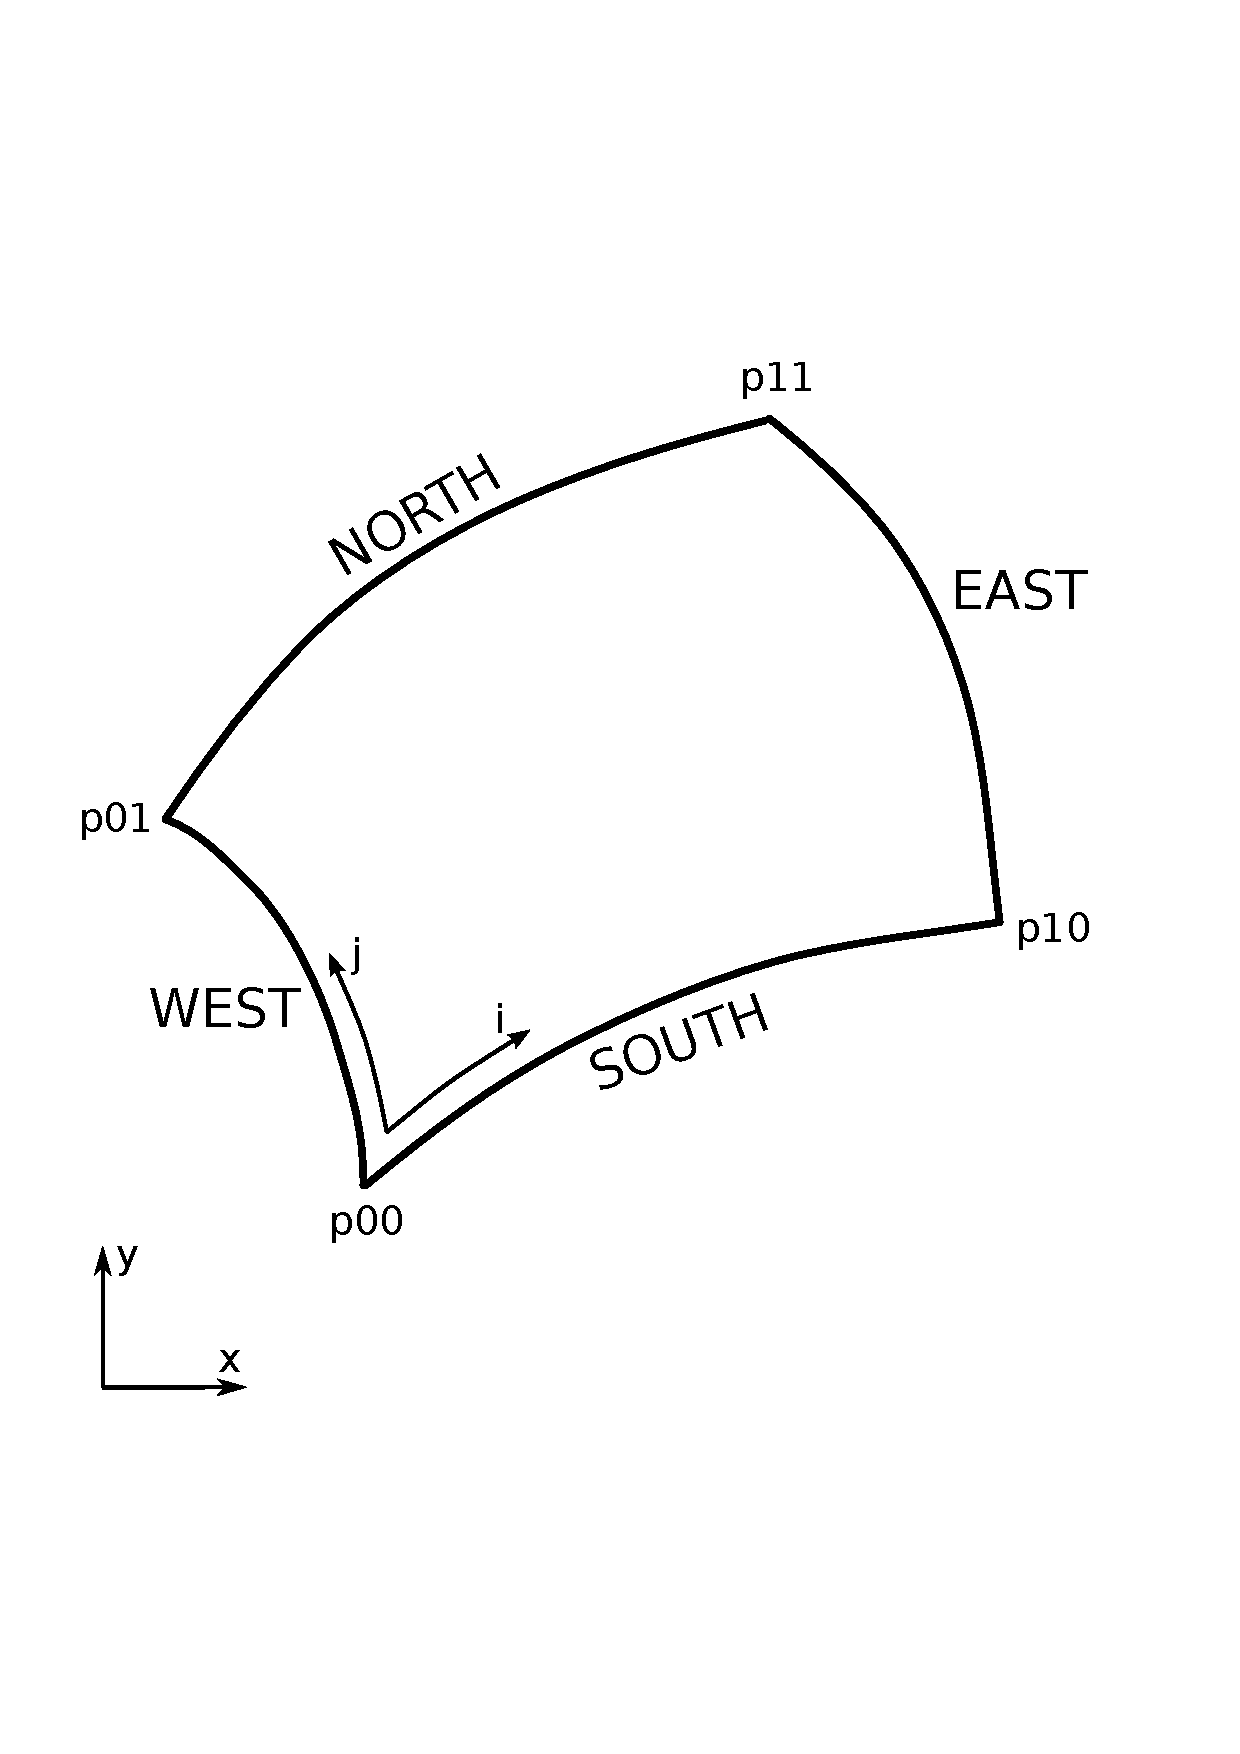
\includegraphics[width=0.5\textwidth,viewport=34 102 524 671,clip=true]{figs/block2d-defn.pdf}
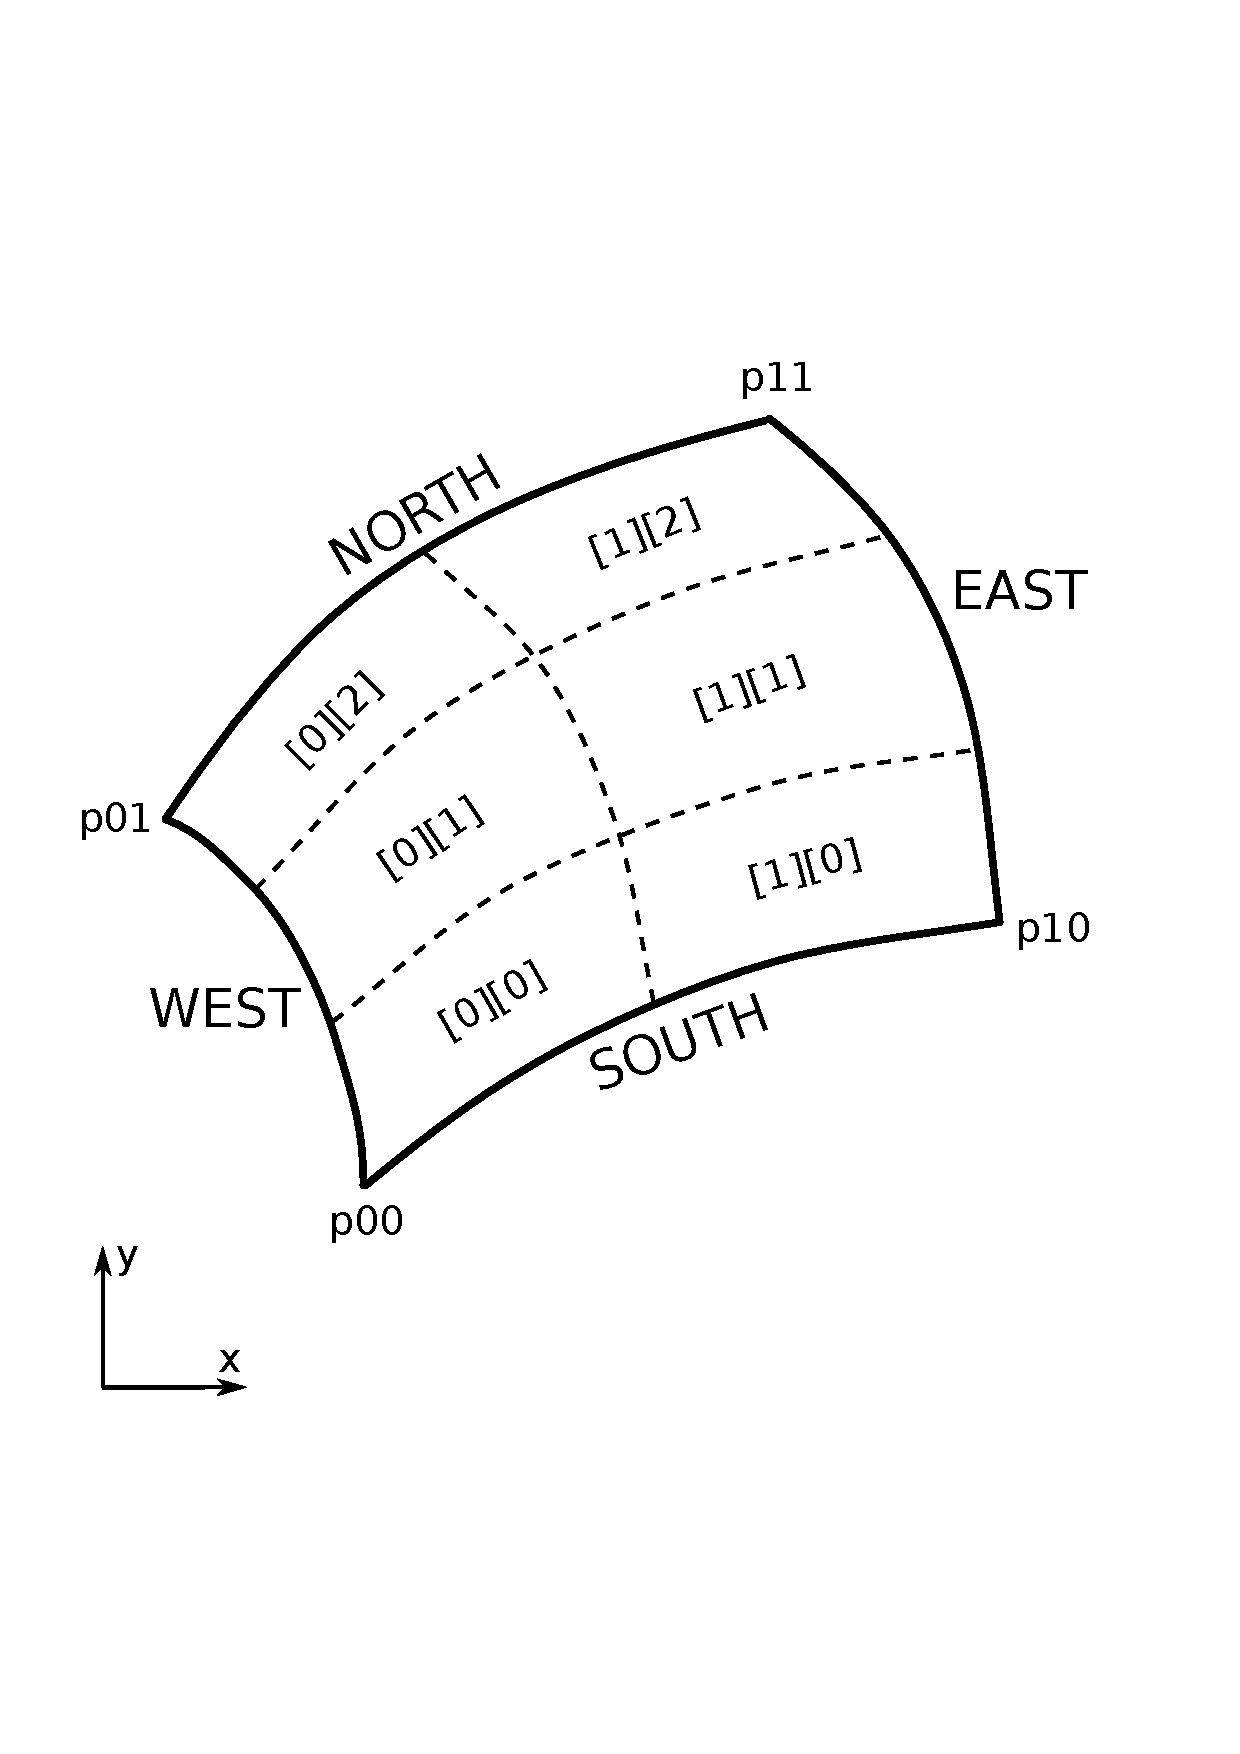
\includegraphics[width=0.5\textwidth,viewport=34 102 524 671,clip=true]{figs/superblock2d-defn.pdf}
}
\caption{A two-dimensional patch containing the structured mesh for a Block2D object (left)
    and a collection of sub-blocks defined via a SuperBlock2D or MultiBlock2D constructor (right).
    The orientations of the bounding paths are important:  
    WEST and EAST paths progress from SOUTH to NORTH;
    SOUTH and NORTH paths progress from WEST to EAST.}
\label{block2d-defn-fig}
\end{figure}

\medskip
To define a block in your input script for a 2D simulation, create a \texttt{Block2D} object as:
\texttt{
\begin{tabbing}
my\_2d\_block = Block2D(\=psurf=None, grid=None, \\
                        \>import\_grid\_file\_name=None, nni=2, nnj=2, \\
                        \>cf\_list=[None,]*4, bc\_list=[SlipWallBC(),]*4, \\
                        \>fill\_condition=None, hcell\_list=[], \\
                        \>xforce\_list=[0,]*4, label="", active=1)
\end{tabbing}\index{block!Block2D}
}
%
\noindent
where the assignment to the name \texttt{my\_2d\_block} allows easy referencing of
the block at later times, say, for adding boundary conditions.
The names of the actual arguments given above match the actual arguments in
the \texttt{e3prep.py} program and these represent\footnote{The
  definitive source is, of course, the \texttt{Block2D} class definition in 
  \texttt{e3\_block.py}\index{module!e3\_block.py}. }:
\begin{itemize}
\item \texttt{psurf}: a region of 2D space bounded by 4 edges.
    Any flat \verb!ParametricSurface! object (from Sec.\,\ref{parametric-surface-sec}) should work.
    This region is often constructed from 4 geometric paths via a call to
    \texttt{make\_patch(north, east, south, west, grid\_type)}\index{make\_patch} where the
    default value for \texttt{grid\_type} is ``TFI'' \textit{i.e.} transfinite interpolation
    or Coons' patch.\index{grid!TFI}\index{grid!transfinite interpolation}
    Another possible form of grid is ``AO'', the area-orthogonality grid.\index{grid!AO}\index{grid!area orthogonality}
    Sometimes, if the blocks are straight-sided quadrilaterals, it will be convenient to define them
    just with the corner points.
    For this case, constructing \verb!CoonsPatch! and \verb!AOPatch! objects directly from the
    corner points may be convenient.
    Providing a constructed \verb!ParametricSurface! is the usual way of specifying the flow domain, 
    which will be discretized using \texttt{nni, nnj, and cf\_list}.
    Note that all geometric elements should have zero values for their z-components when
    doing a 2D flow simulation.
    Since most constructors will have a default value of zero for the z-component, this
    detail can usually be ignored.
\item \texttt{grid}: a \texttt{StructuredGrid} object may be supplied (defaults to None). 
\item \texttt{import\_grid\_file\_name}\index{import\_grid\_file\_name} defaults to None.
  If a name is supplied, this file is read to obtain the grid directly.
  The assumed file format in the legacy (ASCII) VTK format for a structured grid.
\item \texttt{nni} is the number of finite-volume cells in the $i$-index
  direction. See the left part of Figure\,\ref{block2d-defn-fig} for the orientation of the index.
  Note that, when placing one block against another, the blocks must conform in
  \begin{itemize}
    \item the number of cells along corresponding edges
    \item the clustering of those cells along the edges
    \item the path defining the corresponding edges.
  \end{itemize}
  The minimum number of cells is 2, because of the way that the cell-interface values are 
  reconstructed from cell-centred data.
\item \texttt{nnj} is the number of finite-volume cells in the $j$-index direction.
\item \texttt{cf\_list} \label{cflist-item} is an optional list of 4 \texttt{UnivariateFunction} objects
  that specify a (possibly) nonuniform distribution of cells along each particular edge.
  \index{clustering!See univariate function}
  For each object, there is an \texttt{eval(t)} method which returns a transformed (new) value of $t$.
  The options available are:
  \begin{itemize}
    \item \texttt{LinearFunction(m, c)}\index{univariate function!LinearFunction}
      where $t_{new} = m \times t_{old} + c$.
    \item \texttt{LinearFunction2(y0, y1)}\index{univariate function!LinearFunction2}
      where $t_{new} = y0 \times (1-t_{old}) + y1 \times t_{old}$.
    \item \texttt{RobertsClusterFunction(end0, end1, beta)}\index{univariate function!RobertsClusterFunction}
      where the \texttt{end0, end1} integer flags indicate which end (possibly both) we wish to cluster toward.
      The value of \texttt{beta} $> 1.0$ specifies the strength of the clustering, with the clustering
      being stronger for smaller values of \texttt{beta}.
      For example, a value of 1.3 would be relatively weak clustering while a value of 1.01 is quite strong
      clustering.
    \item \texttt{ValliammaiFunction(dL0, dL1, L, n)}\index{univariate function!ValliammaiFunction}
      See Adriaan's source code for definitions.
  \end{itemize}
  See the files \texttt{lib/nm/source/fobject.cxx} and \texttt{lib/nm/source/fobject.hh} for details.
  The order of appearance of boundaries in the list is NORTH, EAST, SOUTH and WEST.
  Note that a full list of 4 items is required.
  If you don't want to specify one (or more) of the items in the list, specify \texttt{None} as that item.
\item \texttt{bc\_list} is an optional list of BoundaryCondition objects,
  as described in Section\,\ref{boundary-conditions-sec}.
  You may omit this list completely, or pass \texttt{None} as any of the items.
  Omitted boundary conditions default to a solid, slip-wall condition.
  These boundary conditions may also be set at a later point in your input script,
  one at a time, either by assigning to individual elements of the the block's \texttt{cf\_list}
  attribute or via the \texttt{set\_BC()} method call described in 
  the Section\,\ref{setting-individual-boundary-conditions-sec}.
  Sometimes, this turns out to be handy.
\item \texttt{fill\_condition} is the \texttt{FlowCondition} object with which to
  define the initial flow state within the volume.
  See Section\,\ref{thermo-flow-sec} for defining a suitable flow condition.
  You may alternatively provide a Python function that supplies the flow properties as
  a function of position or you may use an \texttt{ExistingSolution()} object.
\item \texttt{hcell\_list} is a list of ($i,j$)-tuples specifying which
  cells should be monitored at simulation time.
  Data from the specified cells will be written to a ``history'' file for the
  block and may be used at the postprocessing stage to provide flow data as if
  there was a sensor located in the cell.
\item \texttt{xforce\_list}\index{xforce\_list} is an optional list of zeros/ones that indicate if we
  want the force to be calculated for each of the four edges and written to the 
  \texttt{e3shared.log} log file.
  See the notes in the 20$^o$ cone test case (Section\,\ref{cone20-simple-sec}) for an
  example of how to extract this data from the log file. 
\item \texttt{label} is an optional text label for the block.  This label
  will be embedded in the block definition and some of the postprocessing
  programs may use it.
  For example, the \texttt{e3cgns.py} postprocessing program uses labels to group block boundaries symbolically.
\end{itemize}
Note that, when lists of items are provided for the four boundaries,
the order of the boundaries is NORTH, EAST, SOUTH and WEST.
 

\medskip
When defining large domains and running simulations of a parallel computer, 
it may be convenient to define many Block2D objects with one call.
The first of two constructors for this situation is
\texttt{
\begin{tabbing}
\index{block!SuperBlock2D}
my\_block\_list = SuperBlock2D(\=psurf=None, nni=2, nnj=2, nbi=1, nbj=1, \\
                               \>cf\_list=[None,]*4, bc\_list=[SlipWallBC(),]*4, \\
                               \>fill\_condition=None, hcell\_list=[], label="sblk")
\end{tabbing}
}
\noindent
which generates a single grid over \texttt{psurf} and then subdivided that grid
into \texttt{nbi} $\times$ \texttt{nbj} Block2D sub-blocks.
References to all of these sub-blocks are returned as a list of lists, such that
a particular sub-block may be obtained as \texttt{my\_block\_list.blks[i][j]}.
The second constructor is
\texttt{
\begin{tabbing}
my\_block\_list = MultiBlock2D(\=psurf=None, nni=None, nnj=None, \\
                               \>bc\_list=[SlipWallBC(),]*4, \\
                               \>nb\_w2e=1, nb\_s2n=1, nn\_w2e=None, nn\_s2n=None,\\
                               \>cluster\_w2e=None, cluster\_s2n=None,\\
                               \>fill\_condition=None, label="blk")
\end{tabbing}\index{block!MultiBlock2D}
}
\noindent
which first subdivides the parametric patch into sub-patches and then generates an
individual grid over each sub-patch.
Here, a set of \texttt{nb\_w2e} $\times$ \texttt{nb\_s2n} sub-blocks are generated and, if lists
of integers are provided for \texttt{nn\_w2e} and \texttt{nn\_s2n}, these will be used
as the numbers of cells along the edges of the sub-blocks.
If these lists are not supplied, \texttt{nni} $\times$ \texttt{nnj} cells will be divided
across the sub-blocks.
In both of these constructors, the interior boundaries for the sub-blocks are connected 
(as \texttt{AdjacentBC} boundary conditions).

\medskip
When assembling large numbers of blocks for complex geometries, there is a function
\texttt{
\begin{tabbing}
identify\_block\_connections(\=block\_list=None, exclude\_list=[],\\
                             \>tolerance=1.0e-6)
\end{tabbing}\index{block!identify\_block\_connections}
}
\noindent
that performs a brute-force search for all adjacent blocks and sets \texttt{AdjacentBC}
boundary conditions for pairs of edges that have coinciding corners (to within a given tolerance).
If you don't want the search to be over all blocks generated so far, supply a list to
the \texttt{block\_list} argument.  
Alternatively, supply a list for blocks that should be excluded.

\medskip
In some situations, you may want to manually connect particular blocks.
You can use the function
\texttt{
\begin{tabbing}
connect\_blocks\_2D(\= A, faceA, B, faceB, with\_udf=0, filename=None,\\
                    \> is\_wall=0, sets\_conv\_flux=0, sets\_visc\_flux=0,\\
                    \> check\_corner\_locations=True,\\
                    \> reorient\_vector\_quantities=False,\\
                    \> nA=None, t1A=None, nB=None, t1B=None)
\end{tabbing}\index{block!connect\_blocks\_2D}
}
\noindent
where \texttt{A} and \texttt{B} are references to the individual \texttt{Block2D} objects
and \texttt{faceA} and \texttt{faceB} are their adjoining edges (\texttt{NORTH}, 
\texttt{EAST}, \texttt{SOUTH} or \texttt{WEST}).

\medskip
By default, the function checks that the adjoining corners of the blocks do coincide in space.
If they don't, a warning is issued.
Usually, this is what you want, however, there are times when you really do wish to connect 
the flow for boundaries that are not actually coincident in space.
For an example, see the periodic shear-layer in Sec.\,\ref{periodic-shear-layer-sec}, 
where the ends of a periodic domain are manually connected.
Setting \texttt{check\_corner\_locations=False} turns off the check on corner locations.

\medskip
To handle connections where the boundaries are not aligned, you may specify\\
\texttt{reorient\_vector\_quantities=True} and 
supply nominal vectors for each boundary's unit normal and first tangent.
These nominal vector bases are used to define a rotational transformation 
for the vector flow quantities (\textit{i.e.} velocity and magnetic field) 
that are exchanged between the boundaries.
Such a transformation is useful for turbomachinery flows, where only a sector 
of the full flow field is being simulated and an assumed circumferential periodicity
fills in the remaining detail.

\medskip
Most of the time you can just ignore the default arguments associated with user-defined functions
(\textit{i.e.} \texttt{with\_udf, filename, is\_wall, sets\_conv\_flux, sets\_visc\_flux}).
These are used to implement slowly-opening diaphragms and the like. 

\subsection{Putting a 2D description together}
%
As a motivational example, especially for MECH4480 students of CFD,
consider the construction of a grid around a bottle of \textit{James Boag's Premium}.
Figure\,\ref{the-clustered-bottle-svg-fig} shows the final block arrangement with 
the bottle lying on its side.
You can see the profile of the bottle in the curves from $x$=0 to $x$=0.2 metres.
We model only the upper half plane, with the gas domain being the region around the bottle.
Also, we'll do the modelling in stages, starting with a single block defining a limited 
subregion.

\begin{figure}[htbp]
\begin{center}
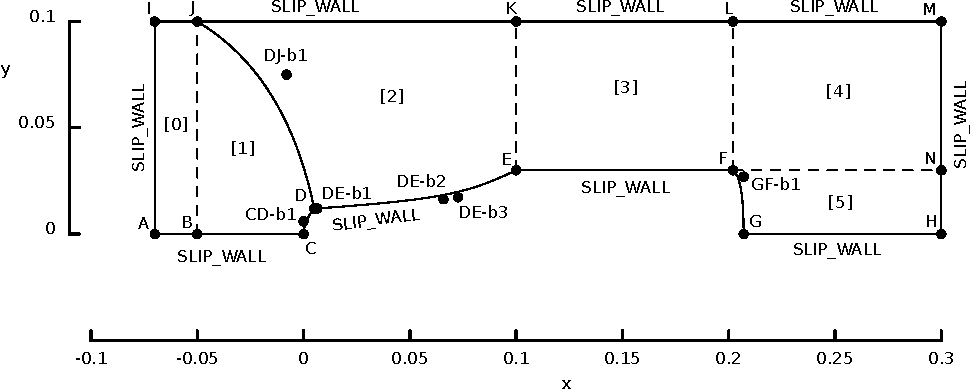
\includegraphics[width=\textwidth]{../2D/beer-bottle/the_clustered_bottle_edited.pdf}
\end{center}
\caption{Schematic diagram of Ingo's beer bottle aligned with the x-axis.
	 This PDF figure was generated from the SVG file with some edits 
	 to move the boundary labels to nicer positions.}
\label{the-clustered-bottle-svg-fig}
\end{figure}

\subsubsection*{Making a simple 2D grid}
%
We start with just block [3] above the main body of the bottle
and define just the 4 nodes E,F,K and L that mark the corners of our
region of interest (Figure\,\ref{the-minimal-grid-fig}).
These are created as \texttt{Nodes} with labels so that they show up in
the generated SVG plot.
A simple way to define the region is to make a patch with the four sides
specified as staight-line paths.
The \texttt{Block2D} is initialized with this patch, the number of cells
in each direction and the initial gas state within the region.

\noindent
\topbar
\lstinputlisting[language={}]{../2D/beer-bottle/the_minimal_grid.py}
\bottombar

\begin{figure}[htbp]
\begin{center}
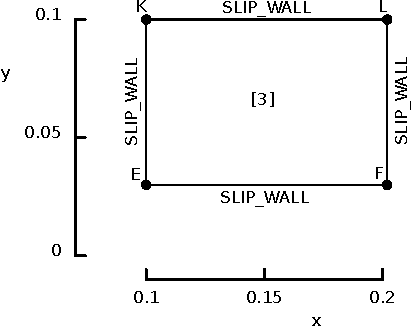
\includegraphics[height=5.5cm]{../2D/beer-bottle/the_minimal_grid_edited.pdf}
\rule{0.5cm}{0cm}
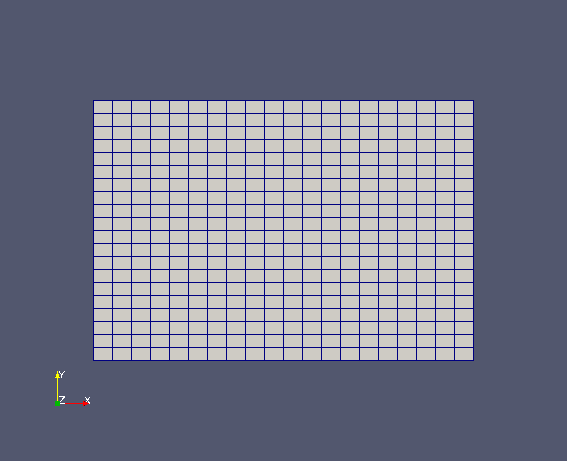
\includegraphics[height=5.5cm]{../2D/beer-bottle/the_minimal_grid.png}
\end{center}
\caption{A single block for a simple subregion from the eventual model 
         of the Ingo's beer bottle.}
\label{the-minimal-grid-fig}
\end{figure}

\subsubsection*{Making a multiblock grid}
%
When making a flow domain that is reasonably complicated, it's probably best
to make a collection of blocks where each block is roughly a quadrilateral,
but with the bounding paths fitted to the curves of the object to be modelled.
Figure~\ref{the-plain-bottle-fig} shows the resulting grid, after dividing 
the full gas-flow region into 6 blocks.

\noindent
\topbar
\lstinputlisting[language={}]{../2D/beer-bottle/the_plain_bottle.py}
\bottombar

\begin{figure}[htbp]
\begin{center}
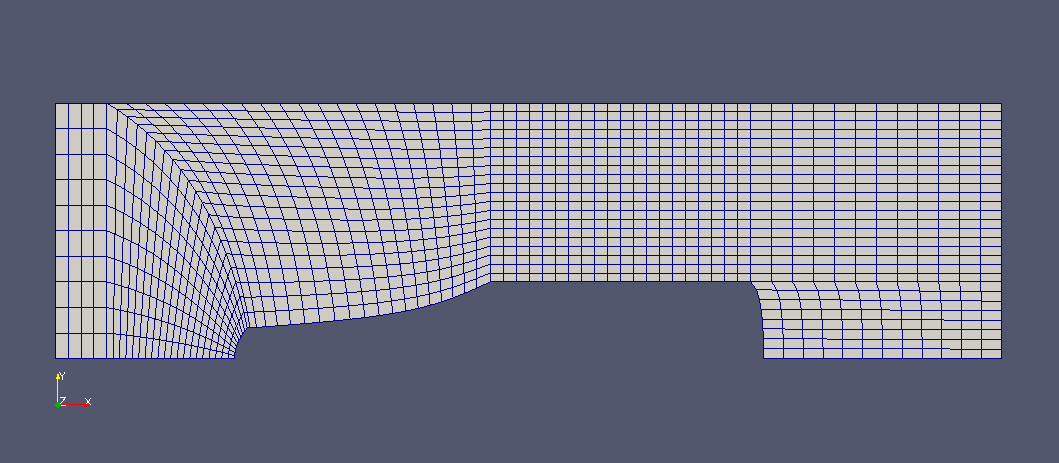
\includegraphics[width=\textwidth]{../2D/beer-bottle/the_plain_bottle.png}
\end{center}
\caption{A multiple-block model of the region around Ingo's beer bottle.}
\label{the-plain-bottle-fig}
\end{figure}

\medskip
Each of the blocks is generated independently of the others.
It is your responsibility to ensure that the common defining edges are 
consistent and that the cell-discretization along each of these edges 
is consistent with the corresponding discretization of any adjacent edge 
of another block.
The first constraint is easy to meet by defining each edge once only and
reusing that path in the definition of different blocks.
Sometimes, the orientation of a pair of blocks and 
the particular directions of the paths within each block means that 
one defining edge needs to be in the opposite sense to the original.
In this case the \texttt{clone()} and \texttt{reverse()} methods may be useful.
The script actually uses the equivalent \texttt{copy(direction=-1)} method call.

\subsubsection*{Improving the grid with clustering}
%
We can now tweak the grid and improve the distribution and shape of the cells
by adjusting the clustering of the points along each of the block edges.
See Figure~\ref{the-clustered-bottle-fig} for the result of the following script.
The partular values used for the strength of the clustering are ad-hoc and some
trial and error has been used to get these particular values.

\medskip
Again, the distribution of points along each edge of each block is computed independently,
so it is the responsibility of the user to ensure that the cells along the 
corresponding edges of adjoining blocks are aligned.
This will require the use of matching clustering functions on these edges.

\noindent
\topbar
\lstinputlisting[language={}]{../2D/beer-bottle/the_clustered_bottle.py}
\bottombar

\medskip
Further improvement of the grid can be made by introducing a layer of blocks around
the bottle surface, so that the cells near the surface can be made always nearly
orthigonal and much more finely clustered toward the surface.
The extra blocks add to the complexity of the input script but provide some decoupling 
with respect to cell number along block edges and allow the fine clustering of cells
toward the bottle surface without greatly increasing 
the cell refinement in other parts of the gas-flow region.
Such a grid would be suited to simulations of viscous flows.

\begin{figure}[htbp]
\begin{center}
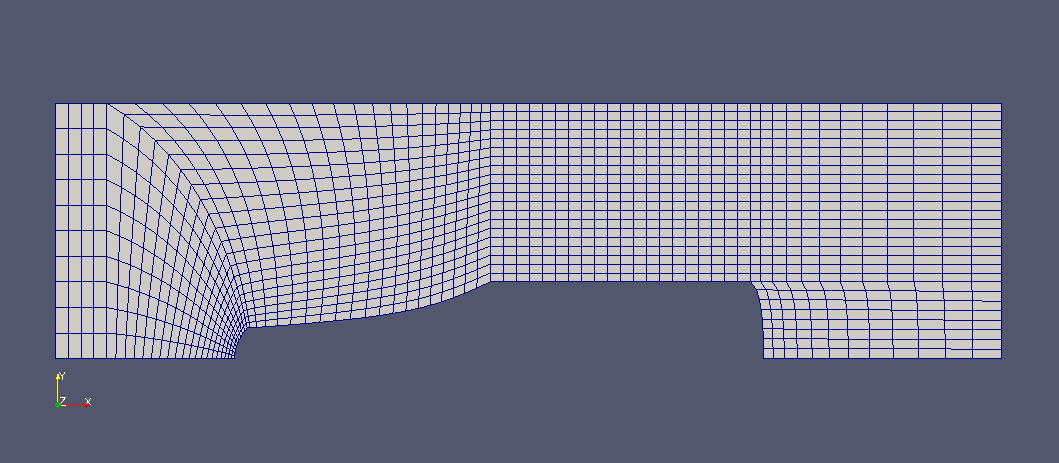
\includegraphics[width=\textwidth]{../2D/beer-bottle/the_clustered_bottle.png}
\end{center}
\caption{An improved multiple-block grid around Ingo's beer bottle.}
\label{the-clustered-bottle-fig}
\end{figure}


%------------------------------------------------------------------
\subsection{Three-dimensional grids}\index{grid!3D}
\label{block3d-sec}
%
In 3D, life is just that bit more complicated with
each block defined by 6 surfaces (NORTH, EAST, SOUTH, WEST, TOP and BOTTOM) 
fitted to the actual surfaces of the domain.
Figure\,\ref{block-defn-fig} shows the ``index-space'' view with cell indices
$i$,$j$ and $k$ taking values $0 \le i < nni$, $0 \le j < nnj$ and 
$0 \le k < nnk$ respectively.\footnote{
  The $i$, $j$ and $k$ indices are related to the $r$, $s$ and $t$ parameters
  used within the 3D geometric functions.
  In some places, the corner points are identified by their ($r,s,t$)
  coordinates.
  For example, in the simple-ramp postprocessing script (section
  \ref{simple-ramp-post-files}), point 0 would be identified as $p000$, point 1
  as $p100$, etc.}
The corner vertices of the block are numbered 1 through 7 as shown.
These points are used in the search to determine block connectivity if the
flow domain is defined as consisting of more than one block.
Subdividing a complex flow domain into simpler subdomains is often done
because the mapping from parametric space to physical space is limited to a
simple transfinite interpolation.

\medskip
To assist in understanding the orientation of the corners, surfaces and indices,
you can build a model block from the development plan in Appendix~\ref{cube-development}.
This should bring back fond memories of kindergarten and primary school, 
at least it did for us.

 
\begin{figure}[htbp]
\mbox{
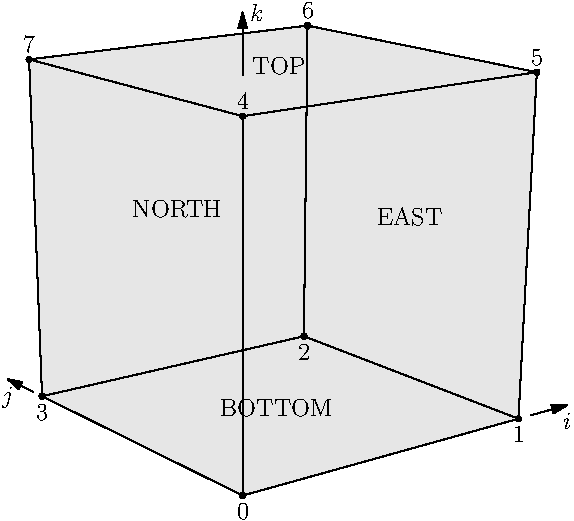
\includegraphics[width=0.5\textwidth]{figs/block3d-defn.pdf}
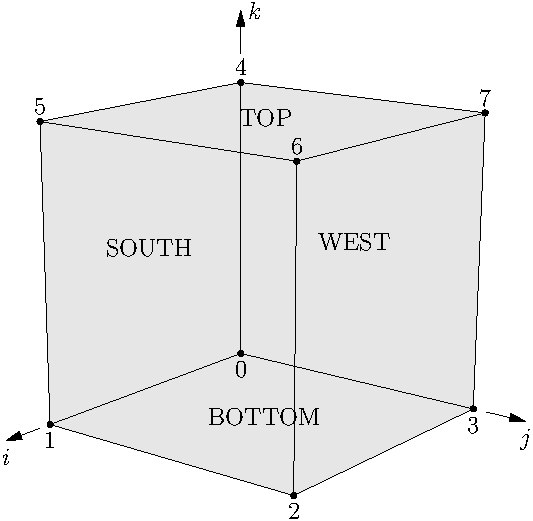
\includegraphics[width=0.5\textwidth]{figs/block3d-defn-2.pdf}
}
\caption{Two views of the hexahedral block containing the structured mesh.
    These figures are ambiguous but each is supposed to show a hollow box
    with the \textit{far} surfaces in each view being labelled.  
    The \textit{near} surfaces are transparent and unlabelled.
    To get your hands on an unambiguous representation, build the debugging cube
    drawn in Appendix\,\ref{cube-development}}.
\label{block-defn-fig}
\end{figure}

\medskip
To define a block in your input script, create a \texttt{Block3D} object as:
\texttt{
\begin{tabbing}
my\_3d\_block = Block3D(\=parametric\_volume=None, grid=None, \\
                        \>import\_grid\_file\_name=None, \\
                        \>nni=None, nnj=None, nnk=None, \\
                        \>cf\_list=[None,]*12, bc\_list=[SlipWallBC(),]*6, \\
                        \>fill\_condition=None, \\
                        \>hcell\_list=None, xforce\_list=[0,]*6, \\
                        \>label="", active=1, omegaz=0.0)
\end{tabbing}\index{block!Block3D}
}
%
\noindent
where the assignment to the name \texttt{my\_3d\_block} allows easy referencing of
the block at later times, say, for adding boundary conditions.
The names of the actual arguments given above match the actual arguments in
the \texttt{e3prep.py} program and these represent\footnote{Again, the
  definitive source is, of course, the \texttt{Block3D} class definition in 
  \texttt{e3\_block.py}. }:
\begin{itemize}
\item \texttt{parametric\_volume}: a region of 3D space bounded by 6 surfaces.
    This is the usual way of specifying the flow domain, which will be discretized 
    using \texttt{nni, nnj, nnk and cf\_list}.
    See the following section for a guide to constructing \texttt{parametric\_volume} objects.
\item \texttt{grid}: a \texttt{StructuredGrid} object may be supplied (defaults to None). 
\item \texttt{import\_grid\_file\_name}\index{import\_grid\_file\_name} defaults to None.
  If a name is supplied, this file is read to obtain the grid directly.
  The assumed file format in the legacy (ASCII) VTK format for a structured grid.
  There is also an external tool (\texttt{p2e.py}) that can be used to convert
  Plot3D format files to Eilmer's native format.
\item \texttt{nni} is the number of finite-volume cells in the $i$-index
  direction as shown in Figure\,\ref{block-defn-fig}.
  This is only used when diecretizing a \texttt{parametric\_volume}.
  When importing or supplying a grid, this data (\texttt{nni, nnj and nnk}) is ignored.
  Note that, when placing one block against another, the blocks must conform in
  \begin{itemize}
    \item the number of cells along corresponding edges
    \item the clustering of those cells along the edges
    \item the path defining the corresponding edges.
  \end{itemize}
\item \texttt{nnj} is the number of finite-volume cells in the $j$-index direction.
\item \texttt{nnk} is the number of finite-volume cells in the $k$-index direction.
\item \texttt{cf\_list} is a list of \texttt{Function} objects
  that specify a (possibly) nonuniform distribution of cells along a
  particular edge of the \texttt{parametric\_volume}.
  The order of the edges is shown in Table\,\ref{edge-list-table}.
  See page~\pageref{cflist-item} for a more complete description of the cluster functions.
\begin{table}
  \caption{Directions for the edges of a \texttt{Block3D} object.}
  \label{edge-list-table}
  \begin{center}
    \begin{tabular}{cccl}
      \hline\hline
      edge & from point & to point & comment \\ 
      \hline
      0  & $p_0$      & $p_1$    & $i$-direction, bottom surface \\
      1  & $p_1$      & $p_2$    & $j$-direction, bottom surface \\
      2  & $p_3$      & $p_2$    & $i$-direction, bottom surface \\
      3  & $p_0$      & $p_3$    & $j$-direction, bottom surface \\
      4  & $p_4$      & $p_5$    & $i$-direction, top surface \\
      5  & $p_5$      & $p_6$    & $j$-direction, top surface \\
      6  & $p_7$      & $p_6$    & $i$-direction, top surface \\
      7  & $p_4$      & $p_7$    & $j$-direction, top surface \\
      8  & $p_0$      & $p_4$    & $k$-direction \\
      9  & $p_1$      & $p_5$    & $k$-direction \\
      10 & $p_2$      & $p_6$    & $k$-direction \\
      11 & $p_3$      & $p_7$    & $k$-direction \\
      \hline \hline
    \end{tabular}
  \end{center}
\end{table}
\item \texttt{bc\_list} is an optional list of BoundaryCondition objects for the 
  six bounding surfaces (\texttt{NORTH, EAST, SOUTH, WEST, TOP, BOTTOM}).
  Available boundary conditions are the same as for Block2D objects and is given
  in Section\,\ref{boundary-conditions-sec}.
  Again, omitted conditions or those specified as \texttt{None} default to
  solid, no-slip walls.
\item \texttt{fill\_condition} is the \texttt{FlowCondition} object with which to
  define the initial flow state within the volume.
  See Section\,\ref{thermo-flow-sec} for defining a suitable flow condition.
  This may also be a callable function that supplies the flow properties as
  a function of position.
\item \texttt{hcell\_list} is a list of ($i,j,k$)-tuples specifying which
  cells should be monitored at simulation time.
  Data from the specified cells will be written to a ``history'' file for the
  block and may be used at the postprocessing stage to provide flow data as if
  there was a sensor located in the cell.
\item \texttt{xforce\_list} is an optional list of zeros/ones that indicate if we
  want the force to be calculated for each of the six surfaces and written to the 
  \texttt{e3shared.log} log file.
  The order of the boundaries is the same as for \texttt{bc\_list}.
\item \texttt{label} is an optional text label for the block.  This label
  will be embedded in the block definition and some of the postprocessing
  programs may use it.
\item \texttt{omegaz} is the rotational speed of the volume about the z-axis.
  This parameter is non-zero only for rotating components of the turbomachine grids.
\end{itemize} 

\medskip
To manually connect particular Block3D objects, you can use the function
\texttt{
\begin{tabbing}
connect\_blocks\_3D(\= A, B, vtx\_pairs, with\_udf=0, filename=None,\\
                    \> is\_wall=0, sets\_conv\_flux=0, sets\_visc\_flux=0)
\end{tabbing}\index{block!connect\_blocks\_3D}
}
\noindent
where \texttt{A} and \texttt{B} are references to the individual \texttt{Block3D} objects
and \texttt{vtx\_pairs} is a list of 4 pairs (tuples) of vertex indices.
For example, the list \texttt{[(3,2),(7,6),(6,7),(2,3)]} specifies a \texttt{NORTH}-to-\texttt{NORTH} connection
with orientation \texttt{0}.
The definitions of all allowable connections is listed near the top of the file \texttt{e3\_block.py}.
You will see that there are \textit{many} more combinations in 3D compared with 2D.

\medskip
As for the 2D grids, there are two composite-block generation functions.
The first takes a volume, grids it and then subdivides the newly generated grid:
\texttt{
\begin{tabbing}
my\_3d\_block = SuperBlock3D(\=parametric\_volume=None, cf\_list=[None,]*12, \\
                        \>fill\_condition=None, \\
                        \>nni=2, nnj=2, nnk=2, \\
                        \>nbi=1, nbj=1, nbk=1, \\
                        \>bc\_list=[SlipWallBC(),]*6, label="sblk", \\
                        \>hcell\_list=None, omegaz=0.0)
\end{tabbing}\index{block!SuperBlock3D}
}
\noindent
where \texttt{nbi}, \texttt{nbi} and \texttt{nbk} are the number of basic blocks in each of the
index directions.
The values for \texttt{nni}, \texttt{nnj} and \texttt{nnk} specify the number of cells for the grid
generated over the whole volume.
The second composite block takes a volume, subdivides that volume and then generates a separate
grid within each subvolume:
\texttt{
\begin{tabbing}
my\_3d\_block = MultiBlock3D(\=parametric\_volume=None, \\
                        \>fill\_condition=None, \\
                        \>nni=None, nnj=None, nnk=None, \\
                        \>nbi=1, nbj=1, nbk=1, \\
                        \>clusteri=None, clusterj=None, clusterk=None, \\
                        \>bc\_list=[SlipWallBC(),]*6, label="blk", \\
                        \>hcell\_list=None, omegaz=0.0)
\end{tabbing}\index{block!MultiBlock3D}
}
\noindent
Here, \texttt{nni}, \texttt{nnj} and \texttt{nnk} may be integer values or lists of integer values.
If they are simple integers, they represent the number of cells over the whole volume.
If they are lists of integers, they specify the number of cells each of the subblocks.
The \texttt{clusteri}, \texttt{clusterj} and \texttt{clusterk} may be lists of cluster functions
that get applied to the subblocks in the respective index directions.

\noindent
Note the the composite-block objects contain a member \texttt{blks} that refers to the list of basic
blocks that form the composite block.
Any further setting of boundary conditions, and the like, 
needs to be done to the individual blocks within this list.
See the input script for the finite-cylinder case (on page\,\pageref{finite-cyl-script}) for an example of this.

\medskip
When assembling large numbers of blocks for complex geometries, the function
\texttt{
\begin{tabbing}
identify\_block\_connections(\=block\_list=None, exclude\_list=[],\\
                             \>tolerance=1.0e-6)
\end{tabbing}\index{block!identify\_block\_connections}
}
\noindent
also works for 3D blocks.
As for 2D blocks, it performs a brute-force search for all adjacent blocks and sets \texttt{AdjacentBC}
boundary conditions for pairs of faces that have coinciding corners (to within a given tolerance).
The rotational orientation of the joined faces is also determined automatically.
If you don't want the search to be over all blocks generated so far, supply a list to
the \texttt{block\_list} argument.  
Alternatively, supply a list for blocks that should be excluded.

\medskip
Be aware that the \texttt{identify\_block\_connections()} function is unaware of the form of the actual paths
or surfaces connecting the corner points. 
It may be that the corners coincide but the paths and surfaces do not conform.
If you want more control over the process of joining blocks, you can manually
connect blocks using the \texttt{connect\_blocks\_3D()} function which makes the logical
connection without looking at the geometric locations of the corners.
This situation might arise, for example, when you want to apply periodic boundary conditions
\index{boundary conditions!periodic} in the cross-stream direction of a flow domain.
Then, the boundaries that you want to connect have corners and faces that really don't coincide.

%-------------------------------------------------------------------
\bigskip
\section{Specifying flow conditions at block boundaries}
\label{boundary-conditions-sec}\index{boundary conditions}
%
The preferred way to set boundary conditions is to assign specific \verb!BoundaryCondition! objects
to the \verb!bc_list! within each constructed \verb!Block2D! or \verb!Block3D! object.
Back in Sections\,\ref{block2d-sec} and \ref{block3d-sec}, it was shown that
the boundary conditions could be specified as a list of \verb!BoundaryCondition! objects 
passed to the constructor of \texttt{Block2D} or \texttt{Block3D} objects, respectively.
You have to provide a list with the correct number of entries, which is 4 for 2D blocks and 6 for 3D blocks.
If you don't have a particular \verb!BoundaryCondition! object for each element of the list,
just specify \verb!None! for the missing entries.

\medskip
Alternatively, \verb!BoundaryCondition! objects can be assigned individually 
to elements of the \verb!bc_list! attribute after block construction.
For example:
\begin{verbatim}
blk_0.bc_list[WEST] = SupInBC(inflow, label="inflow-boundary")
blk_1.bc_list[EAST] = ExtrapolateOutBC(label="outflow-boundary")
\end{verbatim}

\noindent\medskip
Available boundary condition classes include:\index{boundary conditions!list of available}
  \begin{itemize}\index{boundary conditions}
    \item \verb!AdjacentBC(other_block=-1, other_face=-1, orientation=0,!\\
      \verb!reorient_vector_quantities=False,!\\
      \verb!Rmatrix=[1.0, 0.0, 0.0, 0.0, 1.0, 0.0, 0.0, 0.0, 1.0], label='')!\index{boundary conditions!AdjacentBC}\\
      Usually this boundary condition is applied implicitly, by calling the function\\
      \verb!identify_block_connections()!, for cases where one block interfaces with another
      and the block boundaries are cleanly aligned, however, it can be applied manually for cases where you want 
      the flow to be plumbed from on block face into another and the blocks are not geometrically aligned.
      A non-unity transformation matrix, \verb!Rmatrix!, can be provided for cases where the flow vector quantities need to
      be reoriented when they are copied from the other boundary to this one.
    \item \verb!SupInBC(inflow_condition, label='')!\index{boundary conditions!SupInBC} where we want to specify the inflow condition
      that gets copies into the ghost cells each time step.
      The optional \texttt{label} has an empty default value but may be used to group boundary surfaces symbolically
      in the postprocessing stage.
      Paul Petrie-Repar has made use of these labels in his \verb!CGNS! postprocessing program.
    \item \verb!ExtrapolateOutBC(x_order=0, sponge_flag=0, label='')!\index{boundary conditions!ExtrapolateOutBC} where we want a (mostly supersonic) outflow
      condition.
      Flow data is effectively copied (\verb!x_order=0!) or linearly-extrapolated (\verb!x_order=1!)
      from just inside the boundary to the ghost cells just outside the boundary, every time step.
      In subsonic flow, this can lead to unphysical bahaviour.
    \item \verb!SlipWallBC(label='')!\index{boundary conditions!SlipWallBC} where we want a solid wall with no viscous effects.
      This is the default boundary condition where no other condition is specified.
    \item \verb!AdiabaticBC(label='')!\index{boundary conditions!AdiabaticBC} where we want viscous effects to impose no-slip at the wall
      but where there is no heat transfer. 
      Note that we need to set \verb!gdata.viscous_flag = 1! (see Section~\ref{sec:sim-control-parameters}, Viscous effects) 
      to make this boundary condition effective.
    \item \verb!FixedTBC(Twall, label='')!\index{boundary conditions!FixedTBC} where we want viscous effects to impose a no-slip velocity 
      condition and a fixed wall temperature.
      As for the \verb!AdiabaticBC!, we need to set \verb!gdata.viscous_flag = 1! (see Section~\ref{sec:sim-control-parameters}, Viscous effects) 
      to make this boundary condition effective.
    \item \verb!JumpWallBC(Twall, sigma, label='')!\index{boundary conditions!JumpWallBC} where we want viscous effects 
      to impose a partial-slip velocity condition and temperature that approaches a specified wall temperature,
      subject to the limitation of rarefied-gas effects.
      This limitation is specified via the accommodation coefficient, \verb!sigma!.
      As for the \verb!FixedTBC!, we need to set \verb!gdata.viscous_flag = 1! (see Section~\ref{sec:sim-control-parameters}, Viscous effects) 
      to make this boundary condition effective.
    \item \verb!SubsonicInBC(stagnation_condition, mass_flux=0.0, relax_factor=0.05, !\\
      \verb!direction_type='normal', direction_vector=[1.0,0.0,0.0],!\\
      \verb!direction_alpha=0.0, direction_beta=0.0,label='')!\index{boundary conditions!SubsonicInBC} \\
      The flow is assumed subsonic and we specify the stagnation pressure and temperature and 
      a velocity \emph{direction} at the boundary. 
      When applied at each time step, the average local pressure across the block boundary
      is used with the stagnation conditions to compute a stream-flow condition.
      Depending on the value for \verb!direction_type!, the computed velocity's direction can be set 
      \verb!'normal'! to the local boundary, 
      \verb!'uniform'! in direction and aligned with \verb!direction_vector!, 
      \verb!'radial'! in through a cylindrical surface using flow angles \verb!direction_alpha! and \verb!direction_beta!,
      or \verb!'axial'! in through a circular surface using the same flow angles.
      For the case with a nonzero value specified for \verb!mass_flux!, the current mass flux (per unit area)
      across the block face is computed and the nominal stagnation pressure is incremented 
      such that the mass flux across the boundary relaxes toward the specified value.
      The value for \verb!relax_factor! adjusts the rate of convergence for this feedback mechanism.
      Also note, that for multi-temperature simulations, all of the temperatures
      are set to the 0th entry in the temperature array. 
      This should usually be a reasonable physical approximation because this boundary condition
      is typically used to simulate inflow from a reservoir, and stagnated flow in a reservoir 
      has ample time to equilibriate at a common temperature.
      The implementation of this boundary condition may not be time accurate, 
      particularly when large waves cross the boundary, however, it tends to work well in the steady-state limit.
    \item \verb!TransientUniBC(filename, label='')!\index{boundary conditions!TransientUniBC} where we want to specify the time-history of
      the inflow condition.
    \item \verb!StaticProfileBC(filename, n_profile=1, label='')!\index{boundary conditions!StaticProfileBC} where we want to apply a steady-state inflow
       which may vary in space.
    \item \verb!FixedPOutBC(Pout, Tout=300.0, use_Tout=False, x_order=0, label='')!\index{boundary conditions!FixedPOutBC} \\
      is like \verb!ExtrapolateOutBC()! but with a specified back pressure and, possible, a temperature.
      This can be analogous to a vacuum pump that removes gas at the boundary to maintain
      a fixed pressure in the ghost cells.
    \item \verb!UserDefinedBC(filename, is_wall=0, sets_conv_flux=0, sets_visc_flux=0,!\\
          \verb!label='')!\index{boundary conditions!UserDefinedBC}: 
       allows the user to define the ghost-cell flow properties and/or interface fluxes at run time.
       This is done via a set of functions defined by the user, and written in the Lua
       programming language.
       These functions are provided in the file given by \texttt{filename}.
       The flag \verb!is_wall! indicates whether the boundary is to be considered
       a wall for the application of turbulence-model fudges and the like (default 0).
       The flag \verb!sets_conv_flux! indicates whether the user is supplying
       the convective fluxes at the boundary interfaces (default 0), in which case the user-supplied file should
       contain a valid \verb!convective_flux()! function.  
       If not, the internal flux calculator is used together with the supplied ghost-cell data.
       This boundary condition is the Jack of all trades and master of none.
       It can be used to emulate any of the other boundary conditions and then build
       variations, however, it is going to cost quite a lot in computational time.
       Similar to the setting of convective fluxes, the flag \verb!sets_visc_flux!
       indicates whether the user is supplying the viscous fluxes at the boundary interfaces (default 0).
       In this case, the user-supplied file should contain a valid \verb!viscous_flux()! function.
       If not, the internal viscous derivatives are used to compute fluxes based on the supplied interface data.
       See Appendix\,\ref{udf-sec} for the details of setting up this boundary condition.
    \item \verb!AdjacentPlusUDFBC(other_block, other_face, orientation, filename,!\\
          \verb!is_wall=0, sets_conv_flux=0, sets_visc_flux=0,! \\
          \verb!reorient_vector_quantities=False, Rmatrix=None, label='')!\index{boundary conditions!AdjacentPlusUDFBC}: \\
       is a combination of the \texttt{AdjacentBC} and \texttt{UserDefinedBC}.
       At each time step, the flow data is first exchanged, as per the usual
       \texttt{AdjacentBC}.  Then the user-defined functions are applied.
       This is one way of getting fancy boundary conditions, such as slowly-opening diaphragms,
       into the simulation.
    \item \verb!MovingWallBC(r_omega=None, centre=None, v_trans=None,!\\
          \verb!Twall_flag=False, Twall=None, label='')!\index{boundary conditions!MovingWallBC}:
       allows the user to specify a no-slip wall condition where the wall surface has a non-zero velocity.
       Note that this is only for \textit{tangential} velocity at the wall and, to have any effect,
       needs to have \verb!viscous_flag = 1!.
       Values for \verb!r_omega!, \verb!centre! and \verb!v_trans! are specified as tuples of 3-components giving
       the angular-velocity, a point on the axis or rotation and a superimposed translational velocity.
       The actual velocity of a point on the wall is then given by the vector expression 
       $\vec{\omega} \times (\vec{r} - \vec{c}) + \vec{v}_{trans}$,
       where $\vec{r}$ is the point on the wall, 
       $\vec{c}$ is the point on the axis of rotation and $\vec{\omega}$ is the angular velocity.
       This combination allows the setting of planar and cylindrical moving surfaces.
       Optionally, the wall temperature may also be set.  If not, the condition defaults to an adiabatic wall.
    \item \verb!MappedCellBC(ghost_cell_trans_fn=lambda x, y, z: (x, y, z),!\\
          \verb!reorient_vector_quantities=False, !\\
          \verb!Rmatrix=[1.0, 0.0, 0.0, 0.0, 1.0, 0.0, 0.0, 0.0, 1.0],!\\
          \verb!mapped_cell_list=[], label="")!\index{boundary conditions!MappedCellBC}:
       is something like the \verb!AdjacentBC! but with an ad-hoc
       mapping of destination(ghost)-cell location to source-cell location.
  \end{itemize}
Note that, 
when creating these objects in the Python input script, the Python language requires the parentheses
even for the cases where no arguments, such as \texttt{Twall}, are required.
  
\subsection{Setting conditions with setBC (deprecated)}
\label{setting-individual-boundary-conditions-sec}\index{boundary conditions!setting individually}
%
If you have not already set all appropriate boundary conditions through the \verb!bc_list!
argument of the block constructor, you may apply boundary conditions to specific faces 
of a \texttt{Block2D} or \texttt{Block3D} object by calling its method

\noindent
\begin{verbatim}
set_BC(face_name, type_of_BC,
       inflow_condition=None, x_order=0, sponge_flag=None,
       Twall=None, Pout=None, Tout=300.0, use_Tout=False,
       r_omega=None, centre=None, v_trans=None, 
       filename=None, n_profile=1,
       is_wall=0, sets_conv_flux=0, sets_visc_flux=0,
       Twall_flag=False,
       reorient_vector_quantities=False, 
       Rmatrix=[1.0,0.0,0.0, 0.0,1.0,0.0, 0.0,0.0,1.0],
       assume_ideal=0, mdot=None, emissivity=None,
       Twall_i=None, Twall_f=None, t_i=None, t_f=None,
       mass_flux=0.0, p_init=100.0e3, relax_factor=0.05,
       direction_type="normal", direction_vector=[1.0,0.0,0.0],
       direction_alpha=0.0, direction_beta=0.0,
       ghost_cell_trans_fn=lambda x, y, z: (x, y, z),
       I_turb=0.0, u_turb_lam=1.0,
       label='')
\end{verbatim}\index{boundary conditions!set\_BC}

\noindent
and specifying the face and type of boundary condition.
When this function is called, it creates a suitable boundary condition object 
(as discussed in the previous section) and binds it to the appropriate block boundary.
There is no difference in the end result compared with the approach of
specifying the boundary conditions when the block is created. 
\begin{itemize}
  \item \texttt{face\_name}: one of \texttt{NORTH}, \texttt{EAST},
    \texttt{SOUTH}, \texttt{WEST}, \texttt{TOP}, \texttt{BOTTOM}
  \item \texttt{type\_of\_BC}: one of 
    \begin{itemize}
      \item \texttt{ADJACENT}: there is another block abutting this face.
        This boundary condition is usually set by the block-conection functions.
      \item \texttt{SUP\_IN}: supersonic inflow using the
        \texttt{inflow\_condition} properties.
      \item \texttt{EXTRAPOLATE\_OUT}: (assumed) supersonic-outflow where the
        ghost-cell flow properties are copies or extrapolations 
        of the adjacent interior cell properties.
      \item \texttt{SLIP\_WALL}: an inviscid solid wall where the normal
        velocity in the ghost cells is a reflection of the velocity in the
        interoir cell.
      \item \texttt{ADIABATIC}: a no-slip wall where the wall temperature is
        the same as the cell-centre temperature.
      \item \texttt{FIXED\_T}: a no-slip wall where the wall temperature is
        specified by \texttt{Twall} in degrees K.
      \item \texttt{SUBSONIC\_IN}: subsonic inflow where the stagnation
        pressure and temperature is specified and the velocity is taken from
        the interior cell.
      \item \texttt{TRANSIENT\_UNI}: a transient flow condition applied
        uniformly across the face of the block.
      \item \texttt{STATIC\_PROF}: a time-invariant flow condition that has
        spatial variation across the face of the block.
      \item \texttt{FIXED\_P\_OUT}: something like the \texttt{EXTRAPOLATE\_OUT}
        condition with the pressure in the ghost cells set to \texttt{Pout}.
      \item \texttt{RRM}: rescaled and recycled data for Andrew Denman's LES simulations.
      \item \texttt{USER\_DEFINED}: the user-supplied Lua functions are used to
        determine ghost-cell flow properties and or interface fluxes.
        These functions are provided in the file given by \texttt{filename}.
        The flag \texttt{is\_wall} indicates whether the boundary is to be considered
        a wall for the application of turbulence-model fudges and the like (default 0).
        The flag \texttt{sets\_conv\_flux} indicates whether the user is supplying
        the convective fluxes at the boundary interfaces (default 0).  
        If not, the internal flux calculator is used together with the supplied ghost-cell data.
        The flag \texttt{sets\_visc\_flux} indicates whether the user is supplying
        the viscous fluxes at the boundary interfaces (default 0).  
        If not, the internal viscous derivatives are used to compute fluxes based on the supplied interface data.
      \item \texttt{ADJACENT\_PLUS\_UDF}:
      \item \texttt{MOVING\_WALL}: moving wall boundary condition is a solid boundary with no-slip
        but non-zero surface velocity. \verb!r_omega! is a vector to set rotational speed, \verb!centre! is used to
        set the rotational centre and \verb!v_trans! is used to configure the translational velocity of surface.
        Initially, moving wall is a kind of adiabatic wall, if you want to set a fixed temperature condition,
        \verb!Twall_flag! should be \verb!True! temperature to and the temperature specified as \verb!Twall!.
      \item \texttt{MAPPED\_CELL}:
    \end{itemize}
\end{itemize}
You need only specify the other properties that are relevant to the specific boundary condition.

%------------------------------------------------------------------
\bigskip
\section{Special zones and history points}
\label{sec:special-zones}
% 
Zones of heating or cooling may be defined within the flow domain as rectangular (2D) 
or regular hexahedral (3D) patches which are specified by two diagonally-opposite
corners (\verb!point0! and \verb!point1!).
For example, we could specify\\
\verb!HeatZone(qdot, point0, point1, label="")!\index{HeatZone}\\
where \verb!qdot! is the heat addition per unit volume in W/m$^3$.
The corners of each zone are given by the \verb!Vector! values \verb!point0! and \verb!point1!.
In a two-dimensional simulation, 
\verb!point0! corresponds to \verb!p00! in Figure\,\ref{block2d-defn-fig} (on page\,\pageref{block2d-defn-fig}) 
while \verb!point1! corresponds to \verb!p11!, at the opposite corner of the patch.
In three-dimensional simulation, 
\verb!point0! corresponds to \verb!p0! in Figure\,\ref{block-defn-fig} (on page\,\pageref{block-defn-fig}) 
while \texttt{point1} corresponds to \verb!p6! at the diagonally-opposite vertex of the hexahedral block.

\medskip
If the centre of a cell lies within the heat zone, \verb!qdot! is added to
the source term in the energy equation every time step during the simulation. When using
a HeatZone it is necessary to give at least \verb!gdata.heat_time_stop! a positive non-zero
value and \verb!gdata.heat_time_start! and \verb!gdata.heat_factor_increment! can also be modified
as appropriate.
A HeatZone might be used to model the deposition of energy into a small volume from 
a high-power laser, for example.

\medskip
Similarly, zones of reaction are defined with\\
\texttt{ReactionZone(point0, point1, label="")}\index{ReactionZone}\\
where the finite-rate reactions will be allowed to proceed.
Outside of these zones, the finite-rate chemical update will be suppressed 
and the species concentrations will be effectively frozen.
If no such zones are specified, reactions are permitted for the entire flow field.

\medskip
Also, when running turbulent flow simulations, the turbulence model can also be
restricted to being applied to specific zones using\\
\texttt{TurbulenceZone(point0, point1, label="")}\index{TurbulenceZone}\\
The turbulence model (say, the $k-\omega$ model) is active throughout the flow
but its effect on the flow field is masked outside of the \texttt{TurbulenceZone}s.
This is achieved by the code setting the turbulence viscosity and conductivity to zero
for finite-volume cells that fall outside of all regions defined as a \texttt{TurbulenceZone}.
If there a no such defined regions, all of the flowfield may have nonzero turbulence viscosity.

\medskip
As well as being identified by their cell indices when defining a block,
history points can be located by their Cartesian coordinates using:\\
\texttt{HistoryLocation(x, y, z=0.0, i\_offset=0, j\_offset=0, k\_offset=0, label="")}\index{HistoryLocation} \\
where the offset indices allow you to select a cell a known number of cells 
away from another.

%------------------------------------------------------------------
\bigskip
\section{Simulation control parameters}
\label{sec:sim-control-parameters}
\index{configuration parameters}\index{control parameters}
%
A number of other parameters can be set in order to control the behaviour of
the simulation.
These parameters are mainly collected into the \texttt{gdata}
object\footnote{The \texttt{gdata} object is an instance of the \texttt{GlobalData}
  class defined in \texttt{e3prep.py}. Most of the attributes are discussed here,
  however, see the source code for that class for a full list of attributes.} 
which is accessible to the user's input script.
Grouped by theme, the possible attributes include\footnote{Attributes that are stored in the control file\index{control file}
are denoted by a \ddag ~symbol.  The rest go into the config file.\index{config file}}:
\paragraph{Geometry}
\begin{itemize}
\item \texttt{dimensions}: number of geometric dimensions (2 or 3).  
  If unspecified, the default is 2.
\item \texttt{axisymmetric\_flag}: 1=2D-axisymmetric geometry with $x$-axis being the axis of symmetry,
  0=2D-planar geometry, default value 0.
\end{itemize}

\paragraph{Time stepping}
\begin{itemize}
\item \texttt{sequence\_blocks}: 0=normal time iteration on all blocks, 1=integrate one block
  at a time, default value 0.
\item \texttt{dt}\ddag: the initial time step (in seconds) that will be used for the
  first few steps of the simulation process.
  Be careful to set a value small enough for the time-stepping to be stable.
  Since the time stepping is synchronous across all parts of the flow domain,
  this time step size should be smaller than half of the smallest time for a signal
  (pressure wave) to cross any cell in the flow domain. 
  If you are sure that your geometric and boundary descriptions but your simulation
  fails for no clear reason, try setting the initial time step to a very small value.
  For some simulations of viscous hypersonic flow on fine grids, 
  it is not unusual to require time steps to be as small as a nanosecond.
\item \texttt{dt\_max}\ddag: Maximum allowable time step (in seconds),
 default value 1.0e-3.
 Sometimes, especially when strong source terms are at play, the CFL-based time-step 
 determination does not suitably limit the size of the allowable time step.
 This parameter allows the user to limit the maximum time step directly.
\item \texttt{dt\_chem}: suggested time-step for finite-rate chemistry update;
  default value of -1.0 indicates that we want the code to work it out.
\item \texttt{dt\_therm}: default value -1.0.
\item \texttt{gasdynamic\_update\_scheme}\ddag: one of: ``euler'', ``pc'', ``predictor-corrector'',
  ``midpoint'', ``classic-rk3'', ``tvd-rk3'', ``denman-rk3''.
  Default value is ``predictor-corrector''.
  Note that ``pc'' is equivalent to ``predictor-corrector''.
  If you want time-accurate solutions, use a two- or three-stage stepping scheme,
  otherwise, Euler stepping has less computational expense 
  but you may get less accuracy and the code will not be as robust for the same CFL value.
  For example the shock front in the Sod shock tube example is quite noisy for Euler
  stepping at CFL=0.85 but is quite neat with any of the two- or three-stage stepping schemes
  at the same value of CFL.  
  The midpoint and predictor-corrector schemes produce a tidy shock up to CFL = 1.0
  and the rk3 schemes still look tidy up to CFL = 1.2.
\item \texttt{fixed\_time\_step}\ddag: 1=do not change time step from that specified, 
  0=allow time step size to be determined from cell conditions and cfl number, default value 0.
\item \texttt{cfl}\ddag: ratio of the smallest signal time to the actual time step,
  default value 0.5.
\item \texttt{stringent\_cfl}\ddag: 1=use the smallest cross-cell distance in the
  CFL check, 0=use different cell widths in each index direction, default is 0.
\item \texttt{dt\_reduction\_factor}\ddag: if the CFL condition is violated, scale the time-step size
  down by this factor, default value 0.2.
\item \texttt{cfl\_count}: number of time steps between checks of the CFL
  condition, default value 10.
  This check is expensive so we don't want to do it too frequently but, then,
  we have to be careful that the time step does not become unstable.
\item \texttt{max\_time}\ddag: the simulation will be terminated on reaching this
  value of time, default value $1.0 \times 10^{-3}$.
\item \texttt{t0}: starting time for simulation, may be useful to change when restarting from another job,
  default value 0.0.
\item \texttt{max\_step}\ddag: the simulation will be terminated on reaching this
  number of time steps, default value 10.
\item \texttt{dt\_plot}\ddag: the whole flow solution will be written to disk when
  this amount of simulation time has elapsed, default value $1.0 \times 10^{-3}$s.
\item \texttt{dt\_history}\ddag: the history-point data will be written to disk
  when this amount of time has elapsed, default value $1.0 \times 10^{-3}$s.
\end{itemize}

\paragraph{Spatial reconstruction/interpolation}
\begin{itemize}
\item \texttt{x\_order}\ddag: 1=no reconstruction of intra-cell flow properties
  before applying the flux calculator, 2=high-order reconstruction applied, 
  default value 2.
\item \texttt{apply\_limiter\_flag}: 1=apply reconstruction limiter, default value 1.
\item \texttt{extrema\_clipping\_flag}: 1=do extrema clipping at end of 1D scalar reconstruction,
  default value 1.  A value of 0 suppresses clipping.
\item \texttt{interpolation\_type}: string to choose the set of interpolation variables
  to use in the interpolation, options are "rhoe", "rhop", "rhoT", "pT", default value "rhoe".
\end{itemize}

\paragraph{Flux calculator}
\begin{itemize}
\item \texttt{flux\_calc}: selects the flavour of the flux calculator, 
  default value \verb!"adaptive"!. 
  Options are:
  \begin{itemize}
   \item \verb!"riemann"!: An \textit{exact} flux calculator that iteratively solves the Riemann subproblem
    and then constructs the fluxes from the hypothetical interface state.  It's expensive and doesn't behave
    any better than the much cheaper AUSMDV scheme but it does have very little diffusion.  
    The lack of diffusion can cause problems\,\cite{quirk_94a} and it is not recommended for use.
   \item \verb!"ausm"!: A cheap, effective, but sometimes noisy scheme from Ref.\,\cite{liou_steffen_91b}.
   \item \verb!"efm"!: A cheap and very diffusive scheme by Pullin and Macrossan\,\cite{pullin_80,macrossan_89}.
    For most hypersonic flows, it is too diffusive to be used for the whole flow field 
    but it does work very nicely in conjunction with AUSMDV, 
    especially for example, in the shock layer of a blunt-body flow.
   \item \verb!"ausmdv"! A good all-round scheme low-diffusion for supersonic flows.\cite{wada_liou_94a}.
   \item \verb!"adaptive"! A blend\,\cite{quirk_94a} of the low-dissipation AUSMDV scheme 
     for the regions away from shocks
     with the much more diffusive EFM used for cell interfaces near shocks.  
     It seems to work quite reliably for hypersonic flows that are a mix of very strong shocks with
     mixed regions of subsomic and supersonic flow.
     The blend is controlled by the parameters \verb!compression_tolerance! and \verb!shear_tolerance!
     that are described below.
   \item \verb!"ausm_plus_up"!: Implemented from Ref.\,\cite{liou_2006a}.
     It should be accurate and robust for all speed regimes.  
     It is the flux calculator of choice for very low Mach number flows,
     where the fluid behaviour approaches the incompressible limit.
     For best results, you should set the value of \verb!M_inf!.
   \item \verb!"hlle"! The MHD version of the HLLE scheme.
  \end{itemize}  
  The ADAPTIVE scheme is a good all-round scheme that uses AUSMDV away from
  shocks and EFM near shocks.
\item \texttt{compression\_tolerance}: value of relative velocity change (normalised by local sound-speed)
   across a cell-interface that triggers the shock-point detector.  A negative value indicates a compression.
   When the ADAPTIVE flux calculator is used and the shock detector is triggered, the EFM flux calculation
   will be used in place of the default AUSMDV calculation.
   A value of -0.05 seems OK for the sod and cone20 inviscid flow simulations, however,
   a higher value is needed for cases with viscous boundary layers, 
   where it is important to not have too much dissipation in the boundary layer region.
   The default value is -0.30.
\item \texttt{shear\_tolerance}: value of the relative tangential-velocity change 
   (normalised by local sound speed) across a cell-interface that suppresses the use of EFM even if the
   shock detector indicates that EFM should be used for the ADAPTIVE flux calculator.
   The default value is experimentally set at 0.20 to get smooth shocks
   in the stagnation region of bluff bodies.
   A smaller value (say, 0.05) may be needed to get strongly expanding flows to behave 
   when regions of shear are also present.
\item \verb!M_inf!: representative Mach number for the free stream.
   Used by the \verb!AUSM_FLUX_UP! flux calculator. The default value is 0.01.
\end{itemize}

\paragraph{Viscous effects}
\begin{itemize}
\item \texttt{viscous\_flag}: 1=viscous terms are active, 0=inviscid
  simulation, default value 0.
\item \texttt{separate\_update\_for\_viscous\_flag}\ddag: 1=the update 
  for the viscous transport terms are done separately to the convective terms,
  0=the viscous-term updates are initegrated with the explicit update of the convective terms,
  default value 0.
\item \texttt{viscous\_delay}: the time (in seconds) to wait before applying
  the viscous terms.
  This might come in handy when trying to start blunt-body simulations.
\item \texttt{viscous\_factor\_increment}: per-time-step increment of the viscous effects, once
  t\,$>$\,viscous\_delay, default value 0.01.
\item \texttt{diffusion\_flag}: 1=compute multicomponent diffusion of species, default value 0.
\item \texttt{diffusion\_model}: string, default value "None".
\item \texttt{turbulence\_model}: string specifying which model to use, "none", "k\_omega", "baldwin\_lomax",
  default "none".
\item \texttt{turbulence\_prandtl\_number}: default value 0.89
\item \texttt{turbulence\_schmidt\_number}: default value 0.75
\item \texttt{max\_mu\_t\_factor}: turbulent viscosity is limited to laminar viscosity multiplied
  by this factor, default value 300.0. 
\item \texttt{transient\_mu\_t\_factor}: default value 1.0.
\end{itemize}

\paragraph{Thermo-chemistry}
\begin{itemize}
\item \texttt{reacting\_flag}: flag to indicate that the finite-rate chemical
  reactions are active.
  It has a default value of 0, however, it gets set to 1 if the call 
  to \texttt{set\_reaction\_scheme()} is made.
  This is the usual way of setting it.
\item \texttt{reaction\_update}: File name for reaction scheme configuration.
  (More conveniently set by calling \texttt{set\_reaction\_scheme()}.)
\item \texttt{reaction\_time\_start}: time after which finite-rate reactions are allowed to start,
  default value 0.0.
\item \texttt{T\_frozen}: temperature (in degrees K) below which reactions are frozen.
  The default value is 300.0 since most reaction schemes seem to be valid for temperatures
  above this, however, you may have good reasons to set it higher or lower.
  (May also be set in the call to \texttt{set\_reaction\_scheme()}.)
\item \texttt{T\_frozen\_energy}: temperature (in degrees K) below which the energy exchange is skipped.
  The default value is 300.0, however, you may have good reasons to set it higher or lower.
  (May also be set in the call to \texttt{set\_energy\_exchange\_scheme()}.)
\end{itemize}

\paragraph{Miscellaneous}
\begin{itemize}
\item \texttt{title}: a title string that may appear in a number of places.
  For example, in plots made during the postprocessing stage.
\item \texttt{max\_invalid\_cells}: the maximum number of bad cells that will be tolerated on
  decoding conserved quantities.  It this number is exceeded, the simulation will stop. default value 10.
\item \texttt{udf\_source\_vector\_flag}: 1=apply user-defined source terms as supplied in a Lua file,
  default value 0.
\item \texttt{udf\_file}: name of the Lua file for the user-defined source terms, default value "".
\item \texttt{print\_count}\ddag: number of time steps between printing status
  information to the console, default value 20.
\item \texttt{heat\_time\_start}: default value 0.0, in seconds.
  For a description of HeatZones, see Section\,\ref{sec:special-zones}.
\item \texttt{heat\_time\_stop}: a non-zero value indicates that we wish to add heat
  through the HeatZones, default value 0.0, in seconds.
\item \texttt{heat\_factor\_increment}: the fraction of full heat load that will be
  added with each step after $t$=heat\_time\_start, default value 0.01.
\item \texttt{mhd\_flag}: 1=make MHD physics active. default value 0.
\item \texttt{electric\_field\_work\_flag}: 1=make $\vec{u} \cdot \nabla p_e$ sourceterm in the electron energy equation active. default value 0.
\end{itemize}


%------------------------------------------------------------------
\section{Parameters for a 2D sketch of the flow domain}\index{sketch}
%
The \texttt{sketch} object holds parameters that set the view and scale of the
SVG (scalable vector graphic) rendering of the two-dimensional flow domain.
The method
\texttt{
\begin{tabbing}
sketch.window(\=xmin=0.0, ymin=0.0, xmax=1.0, ymax=1.0,\\
              \>page\_xmin=0.05, page\_ymin=0.05, page\_xmax=0.17, page\_ymax=0.17)
\end{tabbing}
}

\noindent
sets the mapping from the lower-left point (xmin,ymin) to 
upper-right point (xmax,ymax) in the simulation space 
to the corresponding points on a display page.
Axes may also be drawn with:\\
\texttt{sketch.xaxis(x0, x1, xtic, y\_offset)} \\
\texttt{sketch.yaxis(y0, y1, ytic, x\_offset)} \\
where small negative values may be given for the offset values, in order to move
the axes clear of the main sketch elements.
Note that these axis parameters are specified in the coordinate system of the simulation space
and that all values are in metres.

% \medskip
% Of course, this sketch environment is only available for 2D simulations.
% For 3D rendering, there is an option for most geometric elements to be rendered as
% Virtual Reality Markup Language (VRML) strings.\index{VRML}  
% These VRML strings may be manually written to a file as part of the user's input script.
